\documentclass[11pt,a4paper]{article}
\usepackage[margin=2.35cm]{geometry}
\usepackage{amsmath,amssymb,bm,graphicx,booktabs,longtable,xcolor,placeins,array,calc,needspace}
\usepackage{newtxtext,newtxmath}
\usepackage[numbers,sort&compress]{natbib}
\usepackage[hidelinks]{hyperref}
\renewcommand{\theequation}{TA\arabic{equation}}
\renewcommand{\thefigure}{TA\arabic{figure}}
\renewcommand{\thetable}{TA\arabic{table}}
\setlength{\emergencystretch}{1em}
\newcommand{\ii}{\mathrm{i}}
\newcommand{\Ai}{\operatorname{Ai}}
\title{Extended Technical Appendix for ``Topological-order-dependent axial advance of a local Stokes domain in Poincar\'e circular Airy beams''}
\author{Youchao Kong, Weiwei Liu, Ze Chen, and Xiyuan Feng}
\date{}
\begin{document}
\maketitle

This appendix contains the extended derivations and full numerical comparisons. Its equation, figure, and table numbering is independent of the accompanying Supplementary Material.


\section{Transverse polarization and the measured signal}
The phasor convention is $\exp(-\ii\omega t)$ and
$\bm e_\pm=(\bm e_x\pm\ii\bm e_y)/\sqrt2$.
For $u=U_{m-P}$, $v=U_{m+P}$, the Cartesian field is
\begin{equation}
E_x=\tfrac12(ue^{\ii(m-P)\theta}+ve^{\ii(m+P)\theta}),\qquad
E_y=\tfrac{\ii}{2}(ue^{\ii(m-P)\theta}-ve^{\ii(m+P)\theta}).
\end{equation}
Direct Jones algebra gives $S_0=|E_x|^2+|E_y|^2$,
$S_1=|E_x|^2-|E_y|^2$, $S_2=2\operatorname{Re}(E_x^*E_y)$, and
$S_3=2\operatorname{Im}(E_x^*E_y)=(|u|^2-|v|^2)/2$.
Thus, where $S_0>0$,
\begin{equation}
\begin{aligned}
s_3&=\frac{|u|^2-|v|^2}{|u|^2+|v|^2}=\sin 2\chi,\\
\psi&=P\theta-\frac{\arg u-\arg v}{2}\pmod\pi.
\end{aligned}
\end{equation}
The second expression is undefined at circular polarization. The orientation
is obtained in the calculations from $\frac12\operatorname{atan2}(S_2,S_1)$
and checked against the circular-channel expression. A common relative
intensity mask $S_0/\max S_0>10^{-9}$ is used for the displayed maps, with
$10^{-12}$ and $10^{-6}$ checked separately. The orientation also requires
$\sqrt{S_1^2+S_2^2}/S_0>10^{-8}$.

For an ideal linear analyzer at angle $\vartheta$,
\begin{equation}
I_\vartheta=\tfrac12S_0[1+V\cos\{2(\vartheta-P\theta)+\delta\}],
\quad V=\frac{2|u||v|}{|u|^2+|v|^2},\quad\delta=\arg u-\arg v.
\end{equation}
For a resolved coherent transverse field, $V^2+s_3^2=1$. Pixel, temporal,
or ensemble averaging need not preserve this equality. A linear analyzer
provides neither the sign of $s_3$ nor the individual circular-channel charges.
For fixed $P=1$, its twofold modulation is common to all $m$. Stokes
polarimetry and circularly matched reference interferometry serve distinct
purposes, as also illustrated in Supplementary Notes 6--7 of Liu
\emph{et al.}\cite{Liu2021} and the detection discussion of Yan
\emph{et al.}\cite{Yan2025}. Here the charge relation is
$m=(q_++q_-)/2$, $P=(q_--q_+)/2$.

Uniform transformations $u\mapsto ue^{\ii\phi_+}$ and
$v\mapsto ve^{\ii\phi_-}$ leave $S_3$ exactly unchanged. They change
$\psi$ by $-(\phi_+-\phi_-)/2$. This control does not remove the effect of
spatial propagation phases on radial amplitudes. In the cached-field check
at $R_0=24$, $\eta=0.70$, $m=1,2,4$, and common planes
$\tau=-0.5,0,1$, the maximum normalized discrepancy between Cartesian and
channel-based $S_3$ was $9.3\times10^{-16}$; the uniform-phase control changed
$S_3$ by less than $6.2\times10^{-16}$ of the plane's maximum $S_0$.

For any common integration region,
\begin{equation}
Q=T\bar p_3,\qquad
T=\frac{P_+^{\rm ROI}+P_-^{\rm ROI}}{P_{\rm in}},\qquad
\bar p_3=\frac{P_+^{\rm ROI}-P_-^{\rm ROI}}{P_+^{\rm ROI}+P_-^{\rm ROI}}.
\end{equation}
The factor $T$ quantifies captured intensity; $\bar p_3$ quantifies its
intensity-weighted circular imbalance. Neither is the arithmetic mean of
$\chi$. A vanishing denominator makes $\bar p_3$ undefined.

\subsection{What $Q$ adds to captured power}
All $Q$, $T$, and $\bar p_3$ comparisons use the same propagated complex
channels, input-power normalization, and ROI for each order. The $Q$ and
$T$ events are nevertheless found independently from each signal's own
first stationary maximum. Define
\begin{equation}
d_m=h_Q(m)-h_T(m),\qquad
E_m=\Delta_Q(m)-\Delta_T(m)=d_1-d_m,
\end{equation}
where $\Delta_X(m)=h_X(1)-h_X(m)$. At $R_0=24$, $\eta=0.7$,
$m=4$, $d_1=0.02626546$ and $d_4=0.02812356$, so the two order
differences are close: $\Delta_Q=0.29196941$, $\Delta_T=0.29382751$,
and $E_4=-0.00185811$. This is a near-common-mode cancellation at that
condition, not a decomposition of the advance into intensity and
polarization percentages. At $R_0=96$ with the same $\eta,m$,
$\Delta_Q=0.07550782$, $\Delta_T=0.09514515$, and
$E_4=-0.01963733$, or $-26.0\%$ of $\Delta_Q$.

All 500 proxy comparisons for $m=2$--6 have defined $Q$ and $T$
half-height events. Their median $|E_m|$ is $0.014207$, the maximum is
$0.250949$, and the median $|E_m/\Delta_Q|$ is $0.13981$. These summary
values establish neither equivalence nor a universal dominance by one
factor. The full machine-readable table includes each single-order event,
$d_m$, both order differences, $E_m$, and status.

Without peak normalization, choose a common $\tau_*=0$ and define
\begin{equation}
\mathcal D_X(\tau)=R_0\ln\frac{X_m(\tau)X_1(\tau_*)}
{X_1(\tau)X_m(\tau_*)}.
\end{equation}
The factorization gives the pointwise identity
$\mathcal D_Q=\mathcal D_T+\mathcal D_{\bar p_3}$. Its maximum numerical
error over all retained valid samples is below $7.4\times10^{-14}$.
For $R_0=24$, $\eta=0.7$, $m=4$, the three slopes at $\tau=0$ are
$-7.897934$, $-7.721899$, and $-0.176036$. At $R_0=96$ they are
$-8.962823$, $-9.630689$, and $+0.667867$. The signed polarization
factor therefore modifies amplitude and can also modify curve shape and
event position.

\begin{table}[htbp]
\centering\scriptsize
\caption{Proxy-boundary comparison of $Q$ and $T$ events. Each signal uses its own first stationary maximum and rising half-height. Here $d_m=h_Q(m)-h_T(m)$, $\Delta_X=h_X(1)-h_X(m)$, and $E_m=\Delta_Q-\Delta_T=d_1-d_m$.}
\label{tab:qt-events}
\begin{tabular}{rrr@{\quad}rrrrrr}
\toprule
$R_0$ & $\eta$ & $m$ & $d_1$ & $d_m$ & $\Delta_Q$ & $\Delta_T$ & $E_m$ & $100E_m/\Delta_Q$ \\
\midrule
24 & 0.35 & 2 & $+0.010670$ & $+0.006233$ & 0.083384 & 0.078947 & $+0.004437$ & $+5.3$ \\
24 & 0.35 & 3 & $+0.010670$ & $-0.008347$ & 0.178589 & 0.159572 & $+0.019017$ & $+10.6$ \\
24 & 0.35 & 4 & $+0.010670$ & $-0.031406$ & 0.284729 & 0.242653 & $+0.042076$ & $+14.8$ \\
24 & 0.70 & 2 & $+0.026265$ & $+0.035752$ & 0.088964 & 0.098450 & $-0.009486$ & $-10.7$ \\
24 & 0.70 & 3 & $+0.026265$ & $+0.035600$ & 0.186557 & 0.195891 & $-0.009334$ & $-5.0$ \\
24 & 0.70 & 4 & $+0.026265$ & $+0.028124$ & 0.291969 & 0.293828 & $-0.001858$ & $-0.6$ \\
96 & 0.35 & 2 & $+0.007388$ & $+0.009786$ & 0.021121 & 0.023519 & $-0.002398$ & $-11.4$ \\
96 & 0.35 & 3 & $+0.007388$ & $+0.009342$ & 0.044790 & 0.046744 & $-0.001954$ & $-4.4$ \\
96 & 0.35 & 4 & $+0.007388$ & $+0.006855$ & 0.070534 & 0.070000 & $+0.000534$ & $+0.8$ \\
96 & 0.70 & 2 & $+0.017295$ & $+0.027256$ & 0.023127 & 0.033089 & $-0.009961$ & $-43.1$ \\
96 & 0.70 & 3 & $+0.017295$ & $+0.033372$ & 0.048474 & 0.064551 & $-0.016077$ & $-33.2$ \\
96 & 0.70 & 4 & $+0.017295$ & $+0.036932$ & 0.075508 & 0.095145 & $-0.019637$ & $-26.0$ \\
\bottomrule
\end{tabular}
\end{table}


\begin{figure}[htbp]
\centering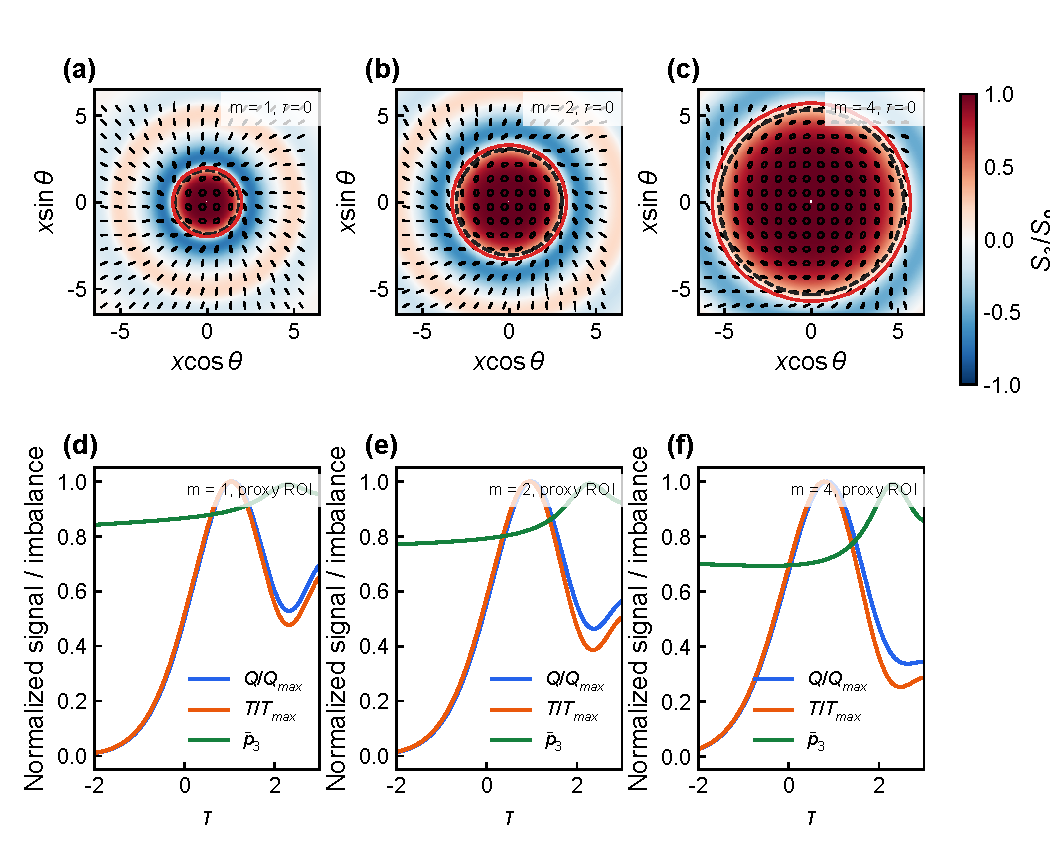
\includegraphics[width=\linewidth]{../figures/polarization_and_observable.pdf}
\caption{Polarization and signal decomposition calculated from complex
reduced R-S channels at $R_0=24$, $\eta=0.70$.
Top: common $\tau=0$ planes, with $x=z\rho/(2kw^3)$.
The color shows $S_3/S_0$; ellipses follow Cartesian Jones fields.
Solid red circles mark the resolved actual $S_3=0$ contour; dashed circles
mark $j'_{m,1}$. Bottom: $Q$ and $T$ separately normalized to their maxima
over the stored interval, together with unscaled $\bar p_3$. The displayed
interval is $-2\leq\tau\leq3$ and the stored interval is $[-3,5]$.
These traces separate captured intensity from polarization composition.}
\end{figure}

\subsection{Short-distance radial mechanism}
For a real radial envelope $f(s)$, $s=\rho/w$, and
$\zeta=z/(kw^2)$, the paraxial radial operator is
$\mathcal L_q=\partial_s^2+s^{-1}\partial_s-q^2s^{-2}$.
At a smooth point away from the axis,
\begin{equation}
U_q=f+\frac{\ii\zeta}{2}\mathcal L_q f
-\frac{\zeta^2}{8}\mathcal L_q^2f+\cdots.
\end{equation}
With $V=s^{-2}$, $[\mathcal D,V]f=4f/s^4-4f'/s^3$ for
$\mathcal D=\partial_s^2+s^{-1}\partial_s$. Hence
\begin{equation}
S_3(s,\zeta)=2mP\zeta^2
\left(\frac{ff'}{s^3}-\frac{f^2}{s^4}\right)+O(\zeta^4).
\label{eq:short-distance-S3}
\end{equation}
The order-dependent current difference at first order is
$j_3=-2mP\,z f^2/(k^2\rho^3)$ in physical coordinates.
Its divergence produces the displayed second-order intensity imbalance.
This is a local smooth-envelope expansion, not an expansion uniform at the
axis or at the Airy caustic. It gives a direct connection between the radial
phase gradient, current, and local circular imbalance. A uniform phase
control removes none of these spatial gradients.

\section{Moving integration regions}
Let $b(z)$ denote a physical radius, distinct from a scaled upper limit.
Leibniz differentiation at fixed physical $\rho$ gives
\begin{equation}
\frac{\mathrm{d}Q_b}{\mathrm{d}z}=\frac{2\pi}{P_{\rm in}}
\left[\int_0^{b(z)}\partial_zS_3\,\rho\,\mathrm{d}\rho
+b(z)b'(z)S_3(b(z),z)\right].
\label{eq:leibniz}
\end{equation}
The physical proxy radius is $b(z)=2kw^3j'_{m,1}/z$, so $b'=-b/z$.
A radius fixed at its value at $z_c$ has $b'=0$. An actual zero contour also
has zero moving-limit term, because its integrand vanishes; its signal still
differs from the proxy integral.

For lossless paraxial propagation, the radial channel currents are
$j_\pm=\operatorname{Im}(U_\pm^*\partial_\rho U_\pm)/(2k)$.
Writing $j_3=j_+-j_-$ gives
\begin{equation}
\frac{\mathrm{d}Q_b}{\mathrm{d}z}=\frac{2\pi b}{P_{\rm in}}
[-j_3(b,z)+b'S_3(b,z)].
\label{eq:current}
\end{equation}
The factor $1/2$ follows from the circular-channel amplitudes in the vector
field. Equation~\eqref{eq:leibniz} is a kinematic identity;
Eq.~\eqref{eq:current} additionally assumes the paraxial wave equation.
It is not a complete Maxwell spin-conservation law and is not assumed exact
for the reduced R-S kernel.
For $R_0=24$, $\eta=0.70$, $m=1,2,4$ and the predeclared interval
$-0.5\leq\tau\leq1.25$, fixed-physical-radius differentiation, direct
Leibniz integration, and the boundary-current expression were compared using
independent Fresnel--Hankel fields. The separate terms are shown in
Fig.~\ref{fig:moving-domain}. The proxy has a nonzero moving-aperture
contribution; the actual zero has a numerically vanishing one. This check
tests the specified paraxial model and does not assert a full-field spin law.
\begin{figure}[htbp]
\centering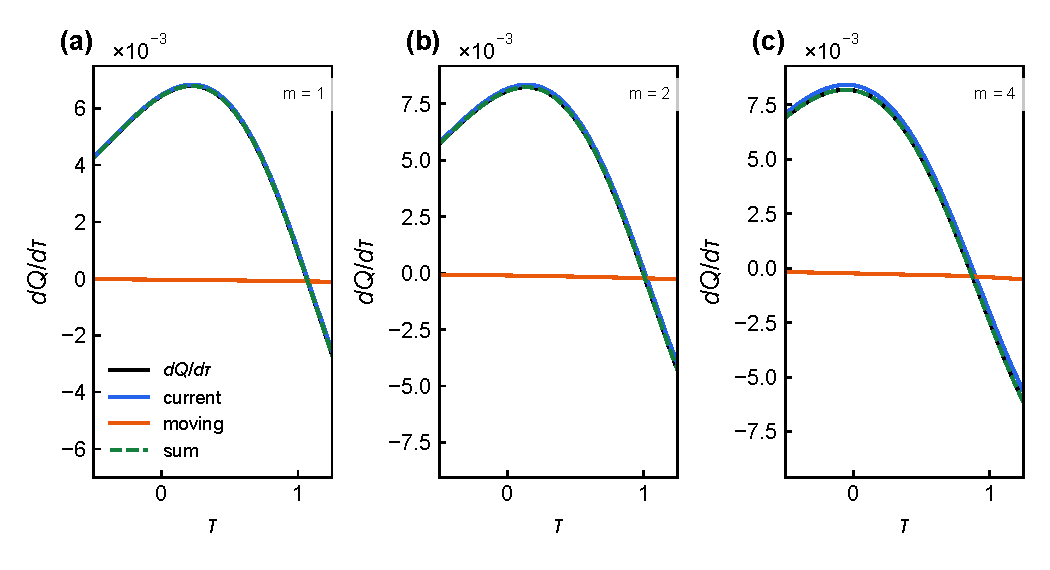
\includegraphics[width=\linewidth]{../figures/moving_domain_decomposition.pdf}
\caption{Derivative of the proxy-domain signal and its paraxial radial-current
and moving-aperture contributions. The dimensionless axis is
$\tau=(z-z_c)/L_c$; plotted derivatives are $\mathrm{d}Q/\mathrm{d}\tau=L_c\,\mathrm{d}Q/\mathrm{d}z$.
All panels use common physical propagation planes. The dashed sum is
independently compared with differentiation of the integrated signal.}
\label{fig:moving-domain}
\end{figure}


\section{Full-amplitude fold expansion}
The main-text normalization uses
$\mathcal U_q^{\rm in}\sim(C_q/2\pi)\int_\Gamma\mathcal F_q e^{\ii(t^3/3+Xt)}\,\mathrm{d}t$,
where
\[
\begin{aligned}
C_q={}&E_0\sqrt{2\pi R_0}(-\ii)^q e^{-\ii\pi/4}
e^{\alpha(R_0-\zeta^2/2)}\\
&\times\exp\!\left\{\ii\left[kz+\zeta(R_0+\alpha^2)/2-\zeta^3/12\right]\right\}.
\end{aligned}
\]
Here $s_c=R_0+(u+\ii\alpha)^2$ and $g=\sqrt{s_c/R_0}$.
The contour runs from $\infty e^{5\pi\ii/6}$ through zero to
$\infty e^{\pi\ii/6}$, with moments
$(2\pi)^{-1}\int_\Gamma t^n e^{\ii(t^3/3+Xt)}\,\mathrm{d}t=(-\ii)^n\Ai^{(n)}(X)$.
The center $t=0$ is the coalescence point at $X=0$, not a stationary point
for general $X$. The common $z$-dependent prefactor is retained throughout
the peak and crossing calculation.

Put $\epsilon=R_0^{-1/2}$, $u_0=\epsilon^{-1}+\epsilon(\tau-\ii\eta)/2$,
and $X_0=-\tau+\ii\eta$. With $u=u_0+t$,
\begin{align}
X&=X_0+\epsilon^2X_2,\qquad X_2=-\tau^2/4+\ii\eta\tau/2,\\
\frac{u}{\sqrt{R_0}}&=1+\epsilon t+\tfrac12\epsilon^2(\tau-\ii\eta),\\
\frac{s_c}{2R_0}&=1+\epsilon t+\tfrac12\epsilon^2(t^2+\tau)
+\tfrac12\epsilon^3t\tau+\tfrac18\epsilon^4\tau^2.
\end{align}
The amplitude $g\sqrt u$ must be expanded together with $J_q(uR)$.
After removal of a common nonzero factor, define
\begin{equation}
\ell_q=J_q+xJ_q',\qquad
n_q=(q^2-x^2+\tfrac12)J_q+xJ_q'.
\end{equation}
Writing $A=\Ai(X_0)$ and using the Airy moments
$t^j\mapsto(-\ii)^j\Ai^{(j)}(X_0)$ gives
\begin{align}
H_q={}&AJ_q-\ii\epsilon A'\ell_q\\
&+\epsilon^2\left[
A\{(\tau/2-\ii\eta/4)J_q-\ii\eta xJ_q'/2\}
-\tfrac12 A''n_q+X_2 A'J_q\right]+O(\epsilon^3).
\end{align}
The squared caustic prefactor contains
$\exp[-2\eta\tau\epsilon-\eta\tau^2\epsilon^3/2]$ and the radial
Jacobian contains $(1+\tau\epsilon^2/2)^{-2}$. A common multiplicative
function of $\tau$ affects individual peaks and crossings and cannot be
deleted before locating them.

At $b_0=j'_{m,1}$, put $J_-=J_{m-1}$, $J_+=J_{m+1}$ and
$I_0=\int_0^{b_0}x(J_-^2-J_+^2)\,\mathrm{d}x=2mJ_m^2(b_0)$.
The complete amplitude obeys
\begin{align}
\int_0^{b_0}x(J_-\ell_--J_+\ell_+)\,\mathrm{d}x&=0,\\
\int_0^{b_0}x(\ell_-^2-\ell_+^2)\,\mathrm{d}x&=0,\\
\int_0^{b_0}x(J_-n_--J_+n_+)\,\mathrm{d}x&=(D_m-\tfrac14)I_0.
\end{align}
Together with $A''=X_0A$, these identities yield
\begin{equation}
\frac{Q_m}{\mathcal N_m}
=f-2\eta\tau f\epsilon+
\epsilon^2\left[(D_m-\tfrac14)\tau f+2\eta^2\tau^2f
+2\operatorname{Re}(A^*A'X_2)\right]+O(\epsilon^3),
\end{equation}
where $f=|A|^2$,
$\mathcal N_m=4\pi^2|E_0|^2w^2\sqrt{R_0}e^{-\eta\sqrt{R_0}}I_0/\mathcal P_{\rm in}$,
and $A'=\Ai'(X_0)$ is an argument derivative, so $\mathrm{d}A/\mathrm{d}\tau=-A'$.
The amplitude $\mathcal N_m$ is distinct from the fourth-order event
coefficient $C_m$. All displayed terms except $D_m\tau f$ are common to
different orders. The finite polynomial calculation through $\epsilon^4$
retains the complex shift of $u_0$, $X_2$, derivatives of $g$, the first
Debye correction, and every intensity cross product. It expands intensity
consistently in $\epsilon$; truncating the field at derivative number $N$
and then squaring is a different operation. The opposite Hankel branch and
the lower spectral endpoint are not included in this local fold series.
Their contribution cannot be assigned to the series remainder without a
separate comparison with the full propagated field.

For reproducibility, let the complete slowly varying amplitude before the
Airy integral be the finite bivariate polynomial
\begin{equation}
P_q(\epsilon,t,x)=\sum_{n=0}^4\sum_j
p_{q,nj}(x)\epsilon^n t^j+O(\epsilon^5).
\end{equation}
The field coefficients used in the calculation are generated by
\begin{equation}
H_{q,n}=\sum_{r=0}^{\lfloor n/2\rfloor}\sum_j
p_{q,n-2r,j}\frac{X_2^r}{r!}(-\ii)^j
\Ai^{(j+r)}(X_0),\qquad 0\le n\le4.
\label{eq:field-recursion}
\end{equation}
This rule includes the $X=X_0+\epsilon^2X_2$ shift and the derivatives of
the full amplitude. If the upper sign denotes $T$ and the lower sign $Q$,
the unprefactored intensity coefficient is
\begin{equation}
I^{T/Q}_{m,n}(x,\tau)=\sum_{a=0}^n\operatorname{Re}
\left[H_{m-1,a}H_{m-1,n-a}^*\ \mathbin{\pm}\
H_{m+1,a}H_{m+1,n-a}^*\right].
\label{eq:intensity-recursion}
\end{equation}
It is integrated with the radial Jacobian and then convolved, order by
order, with the common caustic-prefactor and moving-coordinate Jacobian
series. Equation~\eqref{eq:intensity-recursion} keeps only products whose
total order is $n$; simply squaring a field truncated at a derivative count
also creates terms above the requested intensity order.

Write the selected peak and rising crossing as
\begin{equation}
p_m=p_0+\sum_{n=1}^4p_{m,n}\epsilon^n,\qquad
h_m=h_0+\sum_{n=1}^4h_{m,n}\epsilon^n.
\end{equation}
For a signal $X_m(\tau,\epsilon)=\sum_{n=0}^4x_{m,n}(\tau)\epsilon^n$,
coefficient extraction from $X_m'(p_m)=0$ and
$X_m(h_m)=\gamma X_m(p_m)$ gives
\begin{align}
p_{m,n}&=-\frac{[\epsilon^n]X_m'
(p_0+\sum_{j<n}p_{m,j}\epsilon^j,\epsilon)}{x_{m,0}''(p_0)},\\
h_{m,n}&=\frac{\gamma[\epsilon^n]X_m
(p_0+\sum_{j<n}p_{m,j}\epsilon^j,\epsilon)
-[\epsilon^n]X_m
(h_0+\sum_{j<n}h_{m,j}\epsilon^j,\epsilon)}{x_{m,0}'(h_0)}.
\label{eq:event-recursion}
\end{align}
Here $[\epsilon^n]$ means coefficient extraction after substituting only
previously known event coefficients. The apparently missing $p_{m,n}$ term
in the peak value vanishes because $x_{m,0}'(p_0)=0$. The difference
$c_n=h_{1,n}-h_{m,n}$ gives
\begin{equation}
\Delta_X=c_1R_0^{-1/2}+c_2R_0^{-1}+c_3R_0^{-3/2}
+c_4R_0^{-2}+O(R_0^{-5/2}).
\end{equation}
For the proxy $Q$ event, $c_1=0$ analytically and
$(A_m,B_m,C_m)=(c_2,c_3,c_4)$. For $T$, $c_1$ generally does not vanish.
Table~\ref{tab:qt-formal} gives both observables.

The following command was run from the revision root and reads no
propagation fit data:
\begin{verbatim}
PYTHONPATH=code /usr/bin/python3 code/generate_event_coefficients.py \
  --m 4 --eta 0.7 --observable Q --gamma 0.5 --points 25 --nx 1201 \
  --output theory/generated_coefficients_Q_m4_eta0.7.json
\end{verbatim}
Replacing \texttt{Q} by \texttt{T} generated the corresponding $T$ record.
The $m=4$, $\eta=0.7$ $Q$ result is
$(c_1,c_2,c_3,c_4)=(9.2\times10^{-12},7.91778391,-8.32699328,
15.71031482)$; refinement changed any coefficient by at most
$1.9\times10^{-9}$. For $T$ the values are
$(0.52165323,3.37061776,9.34708065,-45.57713040)$.

\begin{table}[htbp]
\centering\scriptsize
\caption{Non-fitted event-difference coefficients, $\Delta_X=c_1\epsilon+c_2\epsilon^2+c_3\epsilon^3+c_4\epsilon^4+O(\epsilon^5)$, generated directly from the full-amplitude local fold series. The final column is the largest coefficient change when the derivative and radial quadratures are refined.}
\label{tab:qt-formal}
\begin{tabular}{rrcrrrrr}
\toprule
$\eta$ & $m$ & $X$ & $c_1$ & $c_2$ & $c_3$ & $c_4$ & \textbf{refinement} \\
\midrule
0.35 & 2 & Q & $1.51157\times 10^{-13}$ & 2.072213 & $-0.450474$ & $-0.093052$ & $1.74\times 10^{-11}$ \\
0.35 & 3 & Q & $1.50768\times 10^{-12}$ & 4.414678 & $-1.440168$ & 2.587658 & $1.33\times 10^{-11}$ \\
0.35 & 4 & Q & $3.90316\times 10^{-12}$ & 6.972064 & $-2.980978$ & 9.165550 & $2.65\times 10^{-10}$ \\
0.35 & 2 & T & 0.0831185 & 1.387474 & 0.721991 & $-2.173510$ & $9.68\times 10^{-12}$ \\
0.35 & 3 & T & 0.155601 & 2.852249 & 1.413683 & $-4.450309$ & $5.38\times 10^{-11}$ \\
0.35 & 4 & T & 0.221353 & 4.386813 & 2.049090 & $-6.529970$ & $9.61\times 10^{-11}$ \\
0.70 & 2 & Q & $3.4861\times 10^{-13}$ & 2.353296 & $-1.446718$ & 1.103438 & $8.79\times 10^{-10}$ \\
0.70 & 3 & Q & $3.53673\times 10^{-12}$ & 5.013504 & $-4.216432$ & 5.924855 & $1.16\times 10^{-9}$ \\
0.70 & 4 & Q & $9.2073\times 10^{-12}$ & 7.917784 & $-8.326993$ & 15.710315 & $1.86\times 10^{-9}$ \\
0.70 & 2 & T & 0.195882 & 1.034615 & 3.038342 & $-12.028248$ & $2.66\times 10^{-8}$ \\
0.70 & 3 & T & 0.3667 & 2.163520 & 6.177498 & $-27.390268$ & $7.17\times 10^{-8}$ \\
0.70 & 4 & T & 0.521653 & 3.370618 & 9.347081 & $-45.577130$ & $1.30\times 10^{-7}$ \\
0.90 & 2 & Q & $6.05516\times 10^{-13}$ & 2.896903 & $-6.047288$ & 43.080367 & $1.35\times 10^{-8}$ \\
0.90 & 3 & Q & $6.01563\times 10^{-12}$ & 6.171614 & $-14.812476$ & 94.788905 & $1.47\times 10^{-9}$ \\
0.90 & 4 & Q & $1.56808\times 10^{-11}$ & 9.746778 & $-26.230152$ & 154.023590 & $2.30\times 10^{-8}$ \\
0.90 & 2 & T & 0.334402 & $-0.573780$ & 31.524664 & $-638.159910$ & $9.96\times 10^{-7}$ \\
0.90 & 3 & T & 0.626015 & $-1.057104$ & 68.582793 & $-1550.863030$ & $2.59\times 10^{-6}$ \\
0.90 & 4 & T & 0.890545 & $-1.481604$ & 110.834418 & $-2759.205956$ & $5.19\times 10^{-6}$ \\
\bottomrule
\end{tabular}
\end{table}


\section{General boundaries and general polarization index}
For $a=|m-P|$, $c=|m+P|$, define $B=J_a^2-J_c^2$ and
\begin{equation}
I_0(b)=\int_0^b xB(x)\,\mathrm{d}x,\quad
L(b)=\frac{\int_0^b x(\ell_a^2-\ell_c^2)\,\mathrm{d}x}{I_0(b)},\quad
N(b)=\frac{\int_0^b x(J_an_a-J_cn_c)\,\mathrm{d}x}{I_0(b)}.
\end{equation}
The complete first-order integral is
$\int_0^b x(J_a\ell_a-J_c\ell_c)\,\mathrm{d}x=b^2B(b)/2$.
For adjacent orders this reproduces the relative signal correction
\begin{equation}
2\epsilon\frac{\operatorname{Im}(A^*A')}{f}
\frac{bJ_m'(b)}{J_m(b)}.
\end{equation}
Near $b=b_0(1+\delta_b)$,
$bJ_m'(b)/J_m(b)=(m^2-b_0^2)\delta_b+O(\delta_b^2)$.
For a general boundary, both second-order integrals must also be retained.
An integration by parts and the Bessel equation give, for each order $q$,
\begin{align}
\int_0^b x\ell_q^2\,\mathrm{d}x
&=b^3J_q(b)J_q'(b)+\int_0^b x^3J_q^2\,\mathrm{d}x
+(1-q^2)\int_0^b xJ_q^2\,\mathrm{d}x,\\
\int_0^b xJ_qn_q\,\mathrm{d}x
&=(q^2-\tfrac12)\int_0^b xJ_q^2\,\mathrm{d}x
-\int_0^b x^3J_q^2\,\mathrm{d}x+\tfrac12b^2J_q^2(b).
\end{align}

For $P=2,3$, $b_0$ is independently defined as the first nontrivial
positive-to-negative zero of $B$. It is generally not $j'_{m,1}$.
At this root the first-order integral vanishes, but $L$ generally does not.
The order-dependent part of the proxy signal is therefore
\begin{equation}
\epsilon^2\{N\tau f+L|A'|^2\}.
\end{equation}
For example, $(P,m)=(2,2)$ gives $b_0=2.29991033$,
$L=1.74740368$, and $N=-1.78958753$; $(P,m)=(3,3)$ gives
$b_0=2.39837324$, $L=2.22989242$, and $N=-1.76126354$.
These coefficients were computed by direct Bessel integration and checked
against the full-amplitude polynomial expansion before the new $P$-family
propagation. They cannot be replaced by the $P=1$ coefficient $D_m$.
For $m=0$ or $P=0$, the two absolute channel orders are equal and their
balanced radial intensities give identically zero transverse $S_3$.

\section{The moving actual zero}
Write the normalized radial integrand as
$H(x,\epsilon)=H_0(x)+\epsilon H_1(x)+\cdots$, where $H_0=xB$.
Assume $H_0(b_0)=0$ and $H_0'(b_0)<0$. Then
\begin{align}
b_s&=b_0+\epsilon b_1+\cdots,\qquad
b_1=-\frac{H_1(b_0)}{H_0'(b_0)},\\
\int_0^{b_s}H\,\mathrm{d}x-\int_0^{b_0}H\,\mathrm{d}x
&=-\epsilon^2\frac{H_1^2(b_0)}{2H_0'(b_0)}+O(\epsilon^3).
\end{align}
Since $H_1(b_0)=v b_0H_0'(b_0)$ with
$v=\operatorname{Im}(A'/A)$, the root displacement is $b_1=-v b_0$.
For adjacent orders,
$H_0'(b_0)=4m(m^2/b_0^2-1)J_m^2(b_0)$, and the integral correction
divided by $I_0$ is $(3/4-D_m)v^2\epsilon^2$.
Consequently the actual-domain order dependence is
$D_m[\tau-v(\tau)^2]/R_0$. These statements require the same simple root
branch and $A\ne0$. They do not apply through root loss, merger, or a
change in the identity of the first sign-changing root.

\section{Event response and conditioning}
Let a positive signal have a stationary maximum $p$ and preceding rising
crossing $h_\gamma$ satisfying $Q(h_\gamma)=\gamma Q(p)$.
For a small functional perturbation,
\begin{equation}
\delta p=-\frac{\delta Q'(p)}{Q''(p)},\qquad
\delta h_\gamma=\frac{\gamma\delta Q(p)-\delta Q(h_\gamma)}{Q'(h_\gamma)}.
\end{equation}
For a relative perturbation $\epsilon^2 d\,W(\tau)$ of $f$,
the event coefficient is
\begin{equation}
K_\gamma[W]=\frac{\gamma f(p)[W(p)-W(h_\gamma)]}{f'(h_\gamma)}.
\end{equation}
The proxy uses $W=\tau$; the actual adjacent-order domain uses
$W=\tau-v^2$. The general $P$ proxy uses the two functions
$\tau$ and $|A'/A|^2$, with coefficients $N$ and $L$.
For the peak, the proxy coefficient is $-f(p)/f''(p)$.
For a positive-weight centroid over a fixed common window, the coefficient
of a relative linear tilt is its variance in that window. A signed centroid
or an almost vanishing integral has a different interpretation and can be
ill conditioned.

In a statistical measurement, to first order,
\begin{equation}
\operatorname{Var}(\widehat h_\gamma)\simeq
\frac{\gamma^2\sigma_p^2+\sigma_h^2
-2\gamma\operatorname{Cov}(\delta Q_p,\delta Q_h)}{[Q'(h_\gamma)]^2}.
\end{equation}
For $\widehat\Delta=\widehat h_1-\widehat h_m$, its variance additionally
contains $-2\operatorname{Cov}(\widehat h_1,\widehat h_m)$.
This linear formula does not describe branch switching or disappearing
peaks; those events must remain in a full measurement-chain simulation.

\section{Monotonicity and physical scaling paths}
For $m>0$, use the quadratic form
\begin{equation}
q_m[y]=\int_0^1r|y'|^2\,\mathrm{d}r+m^2\int_0^1|y|^2\,\frac{\mathrm{d}r}{r}
\end{equation}
in $L^2((0,1),r\,\mathrm{d}r)$, on its finite-energy domain. On compact positive-order
intervals this domain is common. The natural outer boundary is Neumann,
$y'(1)=0$, and the lowest regular mode is
$y_m(r)=J_m(j'_{m,1}r)$. Its eigenvalue is simple. At the origin
$y_m=O(r^m)$, so the boundary term $r y_m y_m'$ vanishes and both
Hellmann--Feynman integrals converge. Hence
\begin{equation}
\frac{\mathrm{d}}{\mathrm{d}m}(j'_{m,1})^2
=2m\frac{\int_0^1y_m^2\,\mathrm{d}r/r}{\int_0^1r y_m^2\,\mathrm{d}r}>2m,
\end{equation}
which proves $D'(m)<0$. At $m=0$ the constant Neumann mode has eigenvalue
zero, while the first positive derivative zero follows a different indexing
convention; it must not be substituted into this proof.

At fixed $k,w,\eta$, the leading dimensionful advance is
\begin{equation}
\Delta z=\frac{kw^2}{\sqrt{R_0}}\Delta\tau
\sim kw^2 K_\eta(D_1-D_m)R_0^{-3/2}.
\end{equation}
Holding $\alpha$ fixed instead gives $\eta=2\alpha\sqrt{R_0}$ and changes
the axial profile and its event coefficient. When $kw$ is varied at fixed
wavelength, $w=(kw)/k$ must be varied consistently. The accumulated
nonparaxial phase depends on the occupied angular spectrum and propagation
distance, not only on the maximum angle.

\section{Numerical propagation and normalization}
\label{sec:si-numerics}
All dimensional calculations use millimeters internally, with
$\lambda=0.0006328$ mm and baseline $w=0.08$ mm, hence $kw=794.3344257$.
The envelope amplitude is arbitrary because signals are normalized by
$\mathcal P_{\rm in}$. The original 36 beams use
$m=1,2,3$, $\eta=0.35,0.7$, and
$R_0=24,32,40,56,72,96$. The archived calculation and current implementation
agree in all 432 stored comparisons at their saved precision; numerical
convergence is assessed separately below.

\subsection{Independent implementations}
The source-radius-expanded R-S integral is evaluated with composite Simpson
quadrature in $s=r/w$. A kernel coordinate $y$ is defined by
$a=y/(2R_0)$, $c=[1-(a/kw)^2]^{1/2}$,
$\rho=z a/(kw c)$. Its relation to the physical scaled radius is
$x=z\rho/(2kw^3)$; $y$ is only a computational coordinate.
Bessel functions are evaluated directly for each required integer order.
The source phase is split into a separable part and a small correction
containing $c-1$. Four terms in this correction are retained, with an
absolute exponential-remainder bound evaluated for every grid.
The largest stored bound for the tail correction in the main matrix is
$4.18\times10^{-14}$ in field amplitude; it is not a bound on the
event error, which also depends on signal conditioning.

The independent spectral calculation forms
\begin{equation}
H_q(u)=\int_0^\infty s f(s)J_{|q|}(us)\,\mathrm{d}s,\qquad
U_q(r,\zeta)=\int_0^{u_{\max}}u H_q(u)J_{|q|}(ur)
e^{\ii\zeta\Omega(u)}\,\mathrm{d}u,
\end{equation}
where $r=\rho/w$ and the carrier is removed. The rates are
$\Omega_F=-u^2/2$ and
\begin{equation}
\Omega_{\rm exact}=kw\{[(kw)^2-u^2]^{1/2}-kw\}
=-\frac{u^2kw}{[(kw)^2-u^2]^{1/2}+kw}.
\end{equation}
The forward transform uses a logarithmic Hankel grid on
$10^{-6}\leq s\leq10^4$, with $2^{21}$ points below $R_0=192$ and
$2^{22}$ points at larger radius. The logarithmic increment is computed
from the exact endpoint logarithms, avoiding cancellation in a ratio of
adjacent nearly equal grid points. The inverse transform uses uniform
spectral Simpson integration, including the independently integrated
$u=0$ value for $q=0$, rather than a periodic inverse logarithmic transform.
The retained limit is $u_{\max}=\sqrt{24/\alpha}$, below the grazing
region in these comparisons. Production spectral increments are at most
$0.00125$, $0.000625$, and $0.0003125$ for small, intermediate, and
large radii, respectively.

An independent spatial calculation uses the unexpanded first R-S kernel
\begin{equation}
K(d)=Z\,\frac{e^{\ii kw(d-Z)}}{d^2}
\left(\frac1d-\ii kw\right),\quad
d^2=Z^2+s^2+r^2-2sr\cos\varphi,\quad Z=z/w.
\end{equation}
Angular integration projects the required charge, and radial integration
uses an independent Simpson grid. At $\tau=-0.5,0,1$ and
$x=0,1,3,6$, complex fields are compared on all 17 spectral parameter
sets. The largest relative $L^2$ discrepancy is $4.86\times10^{-8}$.
This agreement concerns the same scalar boundary problem. Reduced R-S,
Fresnel, and exact propagation are model comparisons; exact spectral
versus unexpanded R-S differences are implementation comparisons.

\subsection{Extent, sampling, and event convergence}
The production source grid has $\Delta s\leq0.025$ and
$s_{\max}=R_0+\max(45,c/\alpha)$ with
$c=\lceil16+\alpha R_0\rceil$. A smaller preliminary cutoff was found
insufficient at large $R_0$ and strong apodization. Its omitted tail was
added to the cached channels as a complex amplitude; intensities were
then recomputed including interference. Old data are retained separately.
Full-source versus split-tail calculations at three representative cases
change event positions by less than $8\times10^{-9}$.

Independent convergence axes include source increments $0.04,0.025,0.0125$;
observation counts 301, 601, and 1201 for source quadrature and
201, 401, and 801 for
spectral propagation; and axial steps $0.05$, $0.025$, and $0.0125$ when assessed
on the available nested samples. The spectral forward transform is tested
at $2^{21},2^{22},2^{23}$ points and its inverse increment at
$0.000625,0.0003125,0.00015625$ at $R_0=192$, $\eta=0.2$.
Additional source tails increase $c$ by 2 and 4 at
$(24,0.7),(192,0.2),(256,0.9),(256,1.0)$.
Spectral limits $\sqrt{20/\alpha}$, $\sqrt{24/\alpha}$, and
$\sqrt{28/\alpha}$ are compared by coherent annular corrections,
preserving the stored core field. Each refinement changes one numerical
axis at a time. The two annular spectral-extent changes alter
individual half-heights by at most $6.92\times10^{-9}$ over the
three checked parameter sets.

The final source-tail, spectral-sampling, observation, and axial refinements
give maximum half-height and advance changes of $1.47\times10^{-8}$
and $1.88\times10^{-8}$ in the tested set. A cubic-to-quintic locator
comparison at 27 representative beam cases gives a maximum half-height
change $1.14\times10^{-8}$; stationary-peak changes reach
$9.87\times10^{-7}$, demonstrating that crossing and peak accuracies
are different. A Brent tolerance is not a total numerical error estimate.
All detailed values, including earlier failed convergence levels, are
provided in the source-data tables.

The original two-grid advance change, $4.14\times10^{-7}$, omitted source
extent as an independent axis. Extending that extent changes original
single-order positions by up to $1.45\times10^{-5}$ and advances by
$1.71\times10^{-5}$. Original and revised values are tabulated side by
side. Consequently the former grid estimate is not used as the uncertainty
of the revised calculation. Power convergence alone was also insufficient
to establish event convergence.

\begin{table}[t]
\centering\small
\caption{Different error questions, with representative values in
dimensionless $\tau$. Values from distinct rows are not summed.}
\begin{tabular}{p{.30\linewidth}p{.37\linewidth}p{.22\linewidth}}
\toprule
Quantity & Comparison and scope & Value \\
\midrule
Numerical half-height change & Last isolated representative refinements &
$\leq1.47\times10^{-8}$ \\
Numerical advance change & Same refinement set &
$\leq1.88\times10^{-8}$ \\
Source-extent correction & Original 36 beams; maximum advance change &
$1.71\times10^{-5}$ \\
Single-event model difference & Exact minus reduced; $R_0=192,\eta=0.2,m=4$ &
$-0.05850$ \\
Advance model difference & Same beam and reference $m=1$ &
$-6.92\times10^{-6}$ \\
Fresnel minus reduced advance & Same beam; source-radius/paraxial comparison &
$-4.58\times10^{-9}$ \\
Exact minus Fresnel advance & Same beam; exact longitudinal wavenumber &
$-6.92\times10^{-6}$ \\
Boundary-definition change & $+10\%$ radius; $R_0=24,\eta=0.7,m=4$ &
$+0.009368$ \\
Formal-series residual & $\Delta-(A/R_0+B/R_0^{3/2}+C/R_0^2)$;
$R_0=256,\eta=0.7,m=4$ & $1.70\times10^{-5}$ \\
\bottomrule
\end{tabular}
\end{table}

\section{Boundary continuation and event records}
\label{sec:si-root-events}
Each saved complex field supplies 17 regions: 13 fixed scaled factors
$0.8$, $0.85$, $0.9$, $0.925$, $0.95$, $0.975$, $1$, $1.025$,
$1.05$, $1.075$, $1.1$, $1.15$, $1.2$;
the first actual positive-to-negative $S_3$ zero; a physical radius frozen
at the $m$-dependent proxy value at $z_c$; one common physical radius
given by the $m=1$ proxy at $z_c$; and a raised-cosine soft window.
The soft window is unity below $0.95b_0$, zero above $1.05b_0$, and
transitions continuously between them. Channel powers, their sum and
difference, actual roots, and negative-$S_3$ contributions are all saved.
The identity $Q=T\bar p_3$ is evaluated on the same region and input
normalization; it cannot compare regions with different denominators.

To evaluate boundary sensitivity, we compare $0.9b_0$, $b_0$, $1.1b_0$,
and the first actual positive-to-negative zero. For every boundary and every
order, the first stationary maximum and preceding rising half-height are
reselected from that boundary's own signal. The $m=1$ reference uses the
same construction rule as the target order. Table~\ref{tab:four-boundary-full}
covers all six original radii, both original apodizations, and $m=2,3,4$.
It reports signed advances, absolute changes from $b_0$, signed relative
changes, and actual-root event status. The absolute difference remains the
primary quantity when the reference advance is small.

The postprocessing stores separate statuses for the $Q$ pair, the $T$ pair,
their joint comparison, and continuity of the stored selected-root sequence. Among the
actual-root half-height comparisons, 46 have a defined $Q$ order difference
but no joint Q/T comparison because a required $T$ crossing is unavailable.
These records remain valid for Q-only boundary tables and are not silently
reclassified as missing Q events. Selected-root interruptions are reported separately
from event existence.

The wider $0.8b_0$--$1.2b_0$ family is a stress test, not a replacement
protocol. At $R_0=96$, $\eta=0.7$, the $1.2b_0$ advances are
$-0.006342$, $-0.019772$, and $-0.059266$ for $m=2,3,4$, respectively,
whereas the corresponding $b_0$ events remain positive. This reversal is
retained. It cannot be removed by narrowing the axial window or by calling
the changed aperture a numerical error.

The continuity label is a diagnostic of the stored selected-root sequence.
In the main-text display, adjacent finite roots are connected only when their
separation is at most 0.3 in $x$. A missing root or a larger jump interrupts
that sequence; this does not prove a branch exchange or a discontinuity of
the propagated field. Identifying individual branches through such intervals
would require separate root-continuation data.

\begingroup\scriptsize\setlength{\tabcolsep}{3pt}
\begin{longtable}{rrrccccc}
\caption{Four-boundary half-height advances for the original six radii.\label{tab:four-boundary-full}}\\
\toprule
$R_0$ & $\eta$ & $m$ & $0.9b_0$ & $b_0$ & $1.1b_0$ & \textbf{actual zero} & \textbf{status} \\
\midrule
\endfirsthead
\multicolumn{8}{c}{\tablename\ \thetable\ continued}\\
\toprule
$R_0$ & $\eta$ & $m$ & $0.9b_0$ & $b_0$ & $1.1b_0$ & \textbf{actual zero} & \textbf{status} \\
\midrule
\endhead
24 & 0.35 & 2 & \shortstack{0.07356\\(0.00983, $-11.8\%$)} & \shortstack{0.08338\\(0.00000, $+0.0\%$)} & \shortstack{0.09602\\(0.01264, $+15.2\%$)} & \shortstack{0.08677\\(0.00339, $+4.1\%$)} & BR \\
24 & 0.35 & 3 & \shortstack{0.14966\\(0.02893, $-16.2\%$)} & \shortstack{0.17859\\(0.00000, $+0.0\%$)} & \shortstack{0.21896\\(0.04037, $+22.6\%$)} & \shortstack{0.18733\\(0.00874, $+4.9\%$)} & BR \\
24 & 0.35 & 4 & \shortstack{0.22740\\(0.05732, $-20.1\%$)} & \shortstack{0.28473\\(0.00000, $+0.0\%$)} & \shortstack{0.37116\\(0.08643, $+30.4\%$)} & \shortstack{0.30042\\(0.01569, $+5.5\%$)} & BR \\
24 & 0.70 & 2 & \shortstack{0.09082\\(0.00186, $+2.1\%$)} & \shortstack{0.08896\\(0.00000, $+0.0\%$)} & \shortstack{0.08346\\(0.00551, $-6.2\%$)} & \shortstack{0.08429\\(0.00467, $-5.2\%$)} & D \\
24 & 0.70 & 3 & \shortstack{0.18232\\(0.00423, $-2.3\%$)} & \shortstack{0.18656\\(0.00000, $+0.0\%$)} & \shortstack{0.18377\\(0.00278, $-1.5\%$)} & \shortstack{0.18517\\(0.00139, $-0.7\%$)} & BR \\
24 & 0.70 & 4 & \shortstack{0.27369\\(0.01828, $-6.3\%$)} & \shortstack{0.29197\\(0.00000, $+0.0\%$)} & \shortstack{0.30134\\(0.00937, $+3.2\%$)} & \shortstack{0.30218\\(0.01021, $+3.5\%$)} & BR \\
32 & 0.35 & 2 & \shortstack{0.05671\\(0.00594, $-9.5\%$)} & \shortstack{0.06265\\(0.00000, $+0.0\%$)} & \shortstack{0.07004\\(0.00739, $+11.8\%$)} & \shortstack{0.06464\\(0.00199, $+3.2\%$)} & D \\
32 & 0.35 & 3 & \shortstack{0.11505\\(0.01855, $-13.9\%$)} & \shortstack{0.13361\\(0.00000, $+0.0\%$)} & \shortstack{0.15876\\(0.02515, $+18.8\%$)} & \shortstack{0.13913\\(0.00552, $+4.1\%$)} & BR \\
32 & 0.35 & 4 & \shortstack{0.17414\\(0.03785, $-17.9\%$)} & \shortstack{0.21199\\(0.00000, $+0.0\%$)} & \shortstack{0.26759\\(0.05560, $+26.2\%$)} & \shortstack{0.22216\\(0.01017, $+4.8\%$)} & BR \\
32 & 0.70 & 2 & \shortstack{0.07168\\(0.00446, $+6.6\%$)} & \shortstack{0.06722\\(0.00000, $+0.0\%$)} & \shortstack{0.05867\\(0.00856, $-12.7\%$)} & \shortstack{0.06065\\(0.00657, $-9.8\%$)} & D \\
32 & 0.70 & 3 & \shortstack{0.14382\\(0.00314, $+2.2\%$)} & \shortstack{0.14067\\(0.00000, $+0.0\%$)} & \shortstack{0.12855\\(0.01212, $-8.6\%$)} & \shortstack{0.13230\\(0.00838, $-6.0\%$)} & D \\
32 & 0.70 & 4 & \shortstack{0.21550\\(0.00393, $-1.8\%$)} & \shortstack{0.21943\\(0.00000, $+0.0\%$)} & \shortstack{0.20929\\(0.01015, $-4.6\%$)} & \shortstack{0.21400\\(0.00543, $-2.5\%$)} & BR \\
40 & 0.35 & 2 & \shortstack{0.04648\\(0.00375, $-7.5\%$)} & \shortstack{0.05022\\(0.00000, $+0.0\%$)} & \shortstack{0.05470\\(0.00447, $+8.9\%$)} & \shortstack{0.05144\\(0.00121, $+2.4\%$)} & D \\
40 & 0.35 & 3 & \shortstack{0.09419\\(0.01269, $-11.9\%$)} & \shortstack{0.10687\\(0.00000, $+0.0\%$)} & \shortstack{0.12359\\(0.01672, $+15.6\%$)} & \shortstack{0.11056\\(0.00369, $+3.5\%$)} & BR \\
40 & 0.35 & 4 & \shortstack{0.14231\\(0.02682, $-15.9\%$)} & \shortstack{0.16912\\(0.00000, $+0.0\%$)} & \shortstack{0.20755\\(0.03842, $+22.7\%$)} & \shortstack{0.17621\\(0.00709, $+4.2\%$)} & BR \\
40 & 0.70 & 2 & \shortstack{0.05991\\(0.00577, $+10.7\%$)} & \shortstack{0.05413\\(0.00000, $+0.0\%$)} & \shortstack{0.04413\\(0.01000, $-18.5\%$)} & \shortstack{0.04712\\(0.00701, $-13.0\%$)} & D \\
40 & 0.70 & 3 & \shortstack{0.12027\\(0.00706, $+6.2\%$)} & \shortstack{0.11321\\(0.00000, $+0.0\%$)} & \shortstack{0.09645\\(0.01676, $-14.8\%$)} & \shortstack{0.10240\\(0.01082, $-9.6\%$)} & D \\
40 & 0.70 & 4 & \shortstack{0.18018\\(0.00382, $+2.2\%$)} & \shortstack{0.17636\\(0.00000, $+0.0\%$)} & \shortstack{0.15638\\(0.01998, $-11.3\%$)} & \shortstack{0.16493\\(0.01144, $-6.5\%$)} & D \\
56 & 0.35 & 2 & \shortstack{0.03458\\(0.00142, $-4.0\%$)} & \shortstack{0.03600\\(0.00000, $+0.0\%$)} & \shortstack{0.03744\\(0.00144, $+4.0\%$)} & \shortstack{0.03644\\(0.00044, $+1.2\%$)} & D \\
56 & 0.35 & 3 & \shortstack{0.07004\\(0.00641, $-8.4\%$)} & \shortstack{0.07645\\(0.00000, $+0.0\%$)} & \shortstack{0.08434\\(0.00788, $+10.3\%$)} & \shortstack{0.07821\\(0.00176, $+2.3\%$)} & BR \\
56 & 0.35 & 4 & \shortstack{0.10569\\(0.01497, $-12.4\%$)} & \shortstack{0.12066\\(0.00000, $+0.0\%$)} & \shortstack{0.14105\\(0.02039, $+16.9\%$)} & \shortstack{0.12444\\(0.00378, $+3.1\%$)} & BR \\
56 & 0.70 & 2 & \shortstack{0.04599\\(0.00693, $+17.8\%$)} & \shortstack{0.03906\\(0.00000, $+0.0\%$)} & \shortstack{0.02794\\(0.01111, $-28.5\%$)} & \shortstack{0.03232\\(0.00674, $-17.3\%$)} & D \\
56 & 0.70 & 3 & \shortstack{0.09251\\(0.01081, $+13.2\%$)} & \shortstack{0.08171\\(0.00000, $+0.0\%$)} & \shortstack{0.06094\\(0.02077, $-25.4\%$)} & \shortstack{0.06996\\(0.01175, $-14.4\%$)} & D \\
56 & 0.70 & 4 & \shortstack{0.13873\\(0.01154, $+9.1\%$)} & \shortstack{0.12719\\(0.00000, $+0.0\%$)} & \shortstack{0.09833\\(0.02885, $-22.7\%$)} & \shortstack{0.11220\\(0.01499, $-11.8\%$)} & D \\
72 & 0.35 & 2 & \shortstack{0.02782\\(0.00026, $-0.9\%$)} & \shortstack{0.02808\\(0.00000, $+0.0\%$)} & \shortstack{0.02802\\(0.00006, $-0.2\%$)} & \shortstack{0.02816\\(0.00008, $+0.3\%$)} & D \\
72 & 0.35 & 3 & \shortstack{0.05637\\(0.00321, $-5.4\%$)} & \shortstack{0.05957\\(0.00000, $+0.0\%$)} & \shortstack{0.06304\\(0.00347, $+5.8\%$)} & \shortstack{0.06040\\(0.00083, $+1.4\%$)} & D \\
72 & 0.35 & 4 & \shortstack{0.08504\\(0.00886, $-9.4\%$)} & \shortstack{0.09390\\(0.00000, $+0.0\%$)} & \shortstack{0.10523\\(0.01133, $+12.1\%$)} & \shortstack{0.09603\\(0.00213, $+2.3\%$)} & BR \\
72 & 0.70 & 2 & \shortstack{0.03792\\(0.00732, $+23.9\%$)} & \shortstack{0.03060\\(0.00000, $+0.0\%$)} & \shortstack{0.01925\\(0.01135, $-37.1\%$)} & \shortstack{0.02445\\(0.00615, $-20.1\%$)} & D \\
72 & 0.70 & 3 & \shortstack{0.07643\\(0.01237, $+19.3\%$)} & \shortstack{0.06406\\(0.00000, $+0.0\%$)} & \shortstack{0.04194\\(0.02212, $-34.5\%$)} & \shortstack{0.05281\\(0.01125, $-17.6\%$)} & D \\
72 & 0.70 & 4 & \shortstack{0.11477\\(0.01504, $+15.1\%$)} & \shortstack{0.09973\\(0.00000, $+0.0\%$)} & \shortstack{0.06749\\(0.03224, $-32.3\%$)} & \shortstack{0.08451\\(0.01522, $-15.3\%$)} & D \\
96 & 0.35 & 2 & \shortstack{0.02177\\(0.00065, $+3.1\%$)} & \shortstack{0.02112\\(0.00000, $+0.0\%$)} & \shortstack{0.01992\\(0.00120, $-5.7\%$)} & \shortstack{0.02097\\(0.00015, $-0.7\%$)} & D \\
96 & 0.35 & 3 & \shortstack{0.04414\\(0.00065, $-1.4\%$)} & \shortstack{0.04479\\(0.00000, $+0.0\%$)} & \shortstack{0.04481\\(0.00002, $+0.0\%$)} & \shortstack{0.04494\\(0.00015, $+0.3\%$)} & D \\
96 & 0.35 & 4 & \shortstack{0.06662\\(0.00391, $-5.5\%$)} & \shortstack{0.07053\\(0.00000, $+0.0\%$)} & \shortstack{0.07471\\(0.00418, $+5.9\%$)} & \shortstack{0.07140\\(0.00086, $+1.2\%$)} & BR \\
96 & 0.70 & 2 & \shortstack{0.03055\\(0.00742, $+32.1\%$)} & \shortstack{0.02313\\(0.00000, $+0.0\%$)} & \shortstack{0.01193\\(0.01120, $-48.4\%$)} & \shortstack{0.01780\\(0.00532, $-23.0\%$)} & D \\
96 & 0.70 & 3 & \shortstack{0.06173\\(0.01325, $+27.3\%$)} & \shortstack{0.04847\\(0.00000, $+0.0\%$)} & \shortstack{0.02598\\(0.02249, $-46.4\%$)} & \shortstack{0.03839\\(0.01009, $-20.8\%$)} & D \\
96 & 0.70 & 4 & \shortstack{0.09287\\(0.01736, $+23.0\%$)} & \shortstack{0.07551\\(0.00000, $+0.0\%$)} & \shortstack{0.04168\\(0.03383, $-44.8\%$)} & \shortstack{0.06131\\(0.01420, $-18.8\%$)} & D \\
\bottomrule
\end{longtable}
\noindent\footnotesize Each cell is $\Delta\tau_{50}$ on the first line and $(|\Delta-\Delta_{b_0}|,100(\Delta-\Delta_{b_0})/\Delta_{b_0})$ on the second line. D denotes a defined event and BR a defined event whose stored selected-zero sequence contains an interruption; such cases are not used as one smooth asymptotic branch.
\endgroup


Every positive-to-negative root candidate is retained. The trivial vortex
axis zero is excluded. Initial processing uses a relative $S_3$ floor
$10^{-10}$ and a first-cell exclusion; at four critical cases an
independent axis moment determines $U_q/x^{|q|}$ as $x\to0$.
Spline interpolation of this nonsingular quantity in $x^2$ resolves the
root equation without an intensity floor. It detects no additional root
below the original first radial cell in those cases. This is a numerical
test at stated points, not a proof that every dark root is resolvable.

Root jumps larger than $0.3$ in $x$ break the initial event segments.
Continuation identifiers also match all candidates to their linear
predictions between planes; maximum matching distances $0.15,0.3,0.6$
are audited separately. The 1800 records have unchanged event statuses
and half-height differences below $7\times10^{-16}$ relative to the
initial segmentation. These identifiers label numerical continuations and are not
topological invariants. No spline bridges an absent root or an interrupted
branch. The selected event is the earliest interior positive maximum on
a valid segment; all other extrema and crossing candidates remain in the
archive. If the first segment has no valid peak, later valid segments
are examined explicitly and their interval is reported.

An adaptive extent calculation expands the kernel coordinate to $y=32$
and the axial interval to $[-8,12]$ for
three $R_0=24$ cases with $\eta=0.35,0.7,0.9$, four $R_0=96$
cases with $\eta=0.85,0.9,0.925,0.95$, and $(R_0,\eta)=(256,1.0)$.
Cached inner-field planes are reused;
only new axial planes and the outer annulus are propagated. The wider
search does not supply a universal formation event. In particular,
the actual-root $m=4,6$ events remain unavailable on their valid branches
for the tested $R_0=96$, $\eta=0.9,0.925,0.95$ cases, while
$\eta=0.85$ has defined selected events. Failure of a search and
nonexistence on a particular continuous branch are recorded separately
from propagation failure.

For $\eta=0.7$, $m=4$, the formal leading coefficient multiplying
$(D_1-D_4)/R_0$ is $0.80087525$ for the proxy and $0.45152034$ for the
actual-zero boundary. The finite-radius advances can nevertheless be close:
at $R_0=24$ they are $0.291969$ and $0.302175$. Their subleading terms are
still large, and the actual-root record at that radius contains selected-root interruptions.
On the uninterrupted large-radius branch, the effective coefficients
$R_0\Delta/(D_1-D_4)$ reach $0.75488$ for the proxy and $0.54337$ for
the actual zero at $R_0=256$, moving toward distinct limits. At $R_0=16$,
the actual-root $Q$ pair is defined with $\Delta_Q=0.071292$, but its root
records contain selected-root interruptions; the target-order $T$ rising crossing is absent.
The Q point is therefore shown as a selected-root-interruption point and excluded from the
smooth Q convergence sequence, while the joint Q/T comparison is undefined.
The underlying records are in
\texttt{actual\_proxy\_asymptotic\_comparison.csv}.

Rising fractions $0.1$--$0.9$ are evaluated relative to each region's
own first peak. Same-peak FWHM requires the descending half-height
crossing to precede the next local minimum. Among the 10200 main-matrix
region records, 6530 widths meet this condition, 278 cross half-height
only beyond the next minimum, and 3392 lack a pair of crossings.
The latter two groups remain undefined for same-peak width. The earlier,
less restrictive crossing separation is retained as a separate diagnostic.
Common-window centroids use $[-1,2]$ for every order and require a
continuous defined region there; signed weighting and nearly vanishing
integrals are flagged. First-peak conditioning is reported as
$Q(p)/|Q''(p)|$ and half-height conditioning as $Q(p)/|Q'(h)|$.
They measure sensitivity to specified perturbations, not detector error
without a noise model.

Full-curve registration fits a shift and an amplitude over $[-1,2]$
with a shift search $[-1.9,1.9]$ and reports the remaining relative
$L^2$ shape error. Its interpolation domain stays within the saved
$[-3,5]$ interval. Double ratios instead use $\tau_*=0$ and
$\tau\in[-0.5,0.5]$, requiring all four values above
$10^{-8}$ of the larger peak. A measured regression slope is retained
only as a diagnostic; the analytic slope is never replaced by it.

\section{Higher-order, endpoint, and physical-path checks}
\label{sec:si-residuals}
The analytic $A_m,B_m,C_m$ coefficients follow from polynomial algebra
through $\epsilon^4$ and implicit perturbation of the peak and crossing.
All products of lower-order field terms are retained. The next radial
saddle-amplitude correction can be checked independently using the tilted
Airy moment: with $a=\alpha-\ii u$ and $s_*=R_0-a^2$, it is
$-a/(4s_*^2)=\ii\epsilon^3/16-\ii\epsilon^4t/16+\cdots$.
The $\epsilon^3$ part is a common phase, and the normalized intensity
correction at $\epsilon^4$ is $-\operatorname{Re}(A^*A')/8$.
It changes individual fourth-order events but cancels from the
fourth-order order difference. Algebraic checks across orders give
agreement to $2.8\times10^{-13}$. This check does not fit the generated
$m=4$ difference coefficients to propagation data.

The original derivative-number truncation through $N=4$ is retained as
a baseline truncation comparison. It is not identical to a power series truncated
consistently in $\epsilon$. Its original maximum single-event discrepancy
was $1.639\times10^{-3}$, whereas its representative $m=3$ advance
discrepancy was $1.756\times10^{-3}$. Those are approximation errors,
not quadrature errors. The four original figures and 36 parameter cases
define the baseline comparison set.

The formal coefficients are compared without fitting on all available
main-grid radii. Separate least-squares diagnostics fix $A_m$ and fit
$B_m,C_m$ using $R_0\leq96$; the held-out radii are $128,192,256$.
The fit coefficients are labelled empirical and kept separate from
formal coefficients. Near a degenerate Airy maximum, large higher-order
coefficients and finite-radius peaks do not validate a nondegenerate
asymptotic event. At $\eta=1$, the finite-radius proxy events are
retained but no continuation of the simple leading Airy event is asserted.

The fourth-order series at \(\eta=0.35\) does not uniformly improve the
smallest radii and does not locate the intermediate-radius minimum. The
focused calculation in Sec. 14 now closes this residual for \(m=3\): a
compact Airy identity reproduces the full propagated signal, and its
non-fitted expansion through fourteenth order predicts the minimum at
\(R_0=36.37128\), compared with \(36.37130\) for reduced R-S
propagation. The missing fifth- and sixth-order coefficients contain
both field products and nonlinear event terms. This result supersedes
the earlier unresolved attribution for the fixed-proxy \(m=3\) event; it
does not turn a partition-dependent endpoint or Hankel component into an
independently measurable power. The earlier \(m=4\) and other-parameter
comparisons remain finite-order diagnostics with their stated scope.

To examine omitted spectral contributions, the source-axis neighborhood
is smoothly removed from individual Hankel branches below $R_0-10$
and restored through a transition ending at $R_0-8$. A high-frequency
partition is zero below $u_a=\sqrt{R_0}/d$ and one above $2u_a$,
with raised-cosine transition and $d=6,4,3$. The inward and outward
Hankel transforms are propagated coherently; $(1-\chi)H_q$ defines
the low-frequency endpoint component. The remaining high-frequency
field is retained as an explicit remainder. The Debye transform with
8 and 12 terms is checked against direct Hankel-function integration.
Individual components depend on the chosen partition, so their squared
norms are not additive powers and cannot uniquely allocate a physical
mechanism to the residual.

For $\eta=0.7$, $m=4$, $R_0=24$, removing the endpoint component
changes the advance by between approximately $-0.0239$ and $+0.0132$
across the three partitions. At $R_0=256$, the corresponding changes
are between $-4.79\times10^{-5}$ and $+1.04\times10^{-5}$.
The outward component is smaller in field norm at these cases, but
cannot be ignored merely because it has no inward stationary point.
The full coherent sum is partition independent to the implementation
accuracy. Additional $\eta=0.35$ calculations at $R_0=24,32,40,56$
test the nonmonotonic-residual region without changing its data or
analytic coefficients.

The 61 extended parameter jobs contain 276 beams: 40 high-order controls
including $m=1,8,12,16$; 16 small-ring cases at $R_0=8,12$;
88 generalized-$P$ beams; 60 fixed-$\alpha$ beams; and 72 varying-$kw$
beams. High-order searches use a wider radial observation range and
$-6\leq\tau\leq8$. At fixed $\alpha=0.02,0.04,0.07$,
$\eta$ varies with $R_0$ rather than remaining on the principal
asymptotic path. Twenty fixed-$\alpha$ beams have no selected proxy
peak in their stated search interval. They remain in the tables.
No additional validity range is inferred merely from a successful run.

For $P=2,3$, let $h_P$ be the reference event with $m=P$.
The derived leading difference is
\begin{equation}
h_P-h_m=\frac{K_\gamma[\tau](N_{P,P}-N_{P,m})
+K_\gamma[|A'/A|^2](L_{P,P}-L_{P,m})}{R_0}+\cdots.
\end{equation}
At $\eta=0.7$, $P=2,m=4$, its coefficient is $4.61595486$;
the computed difference at $R_0=192$ is $0.02490738$, compared with
the leading $0.02404143$. For $P=3,m=5$, the coefficient is
$4.30569959$ and the corresponding values are $0.02477906$ and
$0.02242552$. These finite-radius discrepancies are retained.
The $m<P$ controls also have positive advances relative to $m=P$
in the sampled set, so monotonicity with $m$ from the adjacent-order
$P=1$ proof is not a general-$P$ statement.

\section{Maxwell completion and longitudinal diagnostics}
\label{sec:si-maxwell}
Let $a=m-1$, $b=m+1$, $\kappa=\sqrt{(kw)^2-u^2}$ and suppress
the common propagation exponential in the integrals below. Preserving
the specified transverse spectrum gives
\begin{align}
E_z(r,\theta)&=\frac{\ii e^{\ii m\theta}}2
\int u^2\frac{H_b-H_a}{\kappa}J_m(ur)e^{\ii\zeta\Omega}\,\mathrm{d}u,\\
V_a(r)&=\int u\left[\frac{\kappa}{kw}H_a+
\frac{u^2(H_a-H_b)}{2kw\kappa}\right]J_a(ur)e^{\ii\zeta\Omega}\,\mathrm{d}u,
\end{align}
with $V_b$ obtained by interchanging $a,b$.
Writing magnetic fields in impedance-scaled units,
\begin{align}
Z_0H_x&=\tfrac\ii2(V_be^{\ii b\theta}-V_ae^{\ii a\theta}),&
Z_0H_y&=\tfrac12(V_ae^{\ii a\theta}+V_be^{\ii b\theta}),\\
Z_0H_z&=-\frac{e^{\ii m\theta}}{2kw}
\int u^2(H_a+H_b)J_m(ur)e^{\ii\zeta\Omega}\,\mathrm{d}u.
\end{align}
The axial Poynting flux obeys
$2Z_0\langle S_z\rangle=\operatorname{Re}(U_aV_a^*+U_bV_b^*)/2$.
This completion differs from projecting a guessed three-component
input and thereby changing the prescribed transverse channels.

The 27 beam/waist cases combine $(R_0,\eta)=(24,0.7),(192,0.2),
(256,0.9)$, $kw=200,800,1600$, and $m=1,4,6$.
Seven common planes $\tau=-1,-0.5,0,0.5,1,1.5,2$ are sampled.
The electric longitudinal fraction is
$\int_{\rm ROI}|E_z|^2/\int_{\rm ROI}(S_0+|E_z|^2)$.
Maximum local fractions use declared bright-pixel masks
$S_0>10^{-9}S_{0,\max}$ and $10^{-6}S_{0,\max}$.
Full-plane retained transverse power, Stokes imbalance, and flux are
reported separately from ROI quantities. The retained transverse power
agrees with the incident scalar normalization to approximately $10^{-9}$
in the checked cases. Apparent remote FFTLog wrap tails are not interpreted
as physical grazing-angle content.

At $R_0=256$, $\eta=0.9$, $kw=800$, the largest sampled relative
ROI axial-flux correction over the three orders is approximately
$1.91\times10^{-4}$. The sampled maxima of the longitudinal electric
fraction across the three physical cases rise from
$3.37\times10^{-5}$--$3.70\times10^{-4}$ at $kw=800$ to
$5.40\times10^{-4}$--$5.77\times10^{-3}$ at $kw=200$.
Small values in these cases do not establish a universal bound near
dark pixels, high orders, or tighter focusing.

Independent Cartesian spectral integration enforces
$\bm k\cdot\widetilde{\bm E}=0$ and
$Z_0\widetilde{\bm H}=\bm k\times\widetilde{\bm E}/k$ directly.
Angular resolutions 64,128,256 agree with the radial recurrence formulas
at matched quadrature points to relative $E,H$ error below
$1.4\times10^{-12}$ and relative $E_z$ error below $6.3\times10^{-12}$.
Comparison to stored interpolated radial fields instead gives errors
up to $1.48\times10^{-7}$, which include interpolation and differing
spectral increments. Operator verification and grid verification are
therefore reported separately.

\section{Input mismatch and two-dimensional controls}
\label{sec:si-inputs}
The input-tolerance study uses $R_0=24,96$, $\eta=0.35,0.7$,
$m=1,2,4$ on $[-8,8]$. Signed power imbalance weights the two
channels by $\sqrt{1+\delta}$ and $\sqrt{1-\delta}$, with
$\delta=\pm0.005,\pm0.01,\pm0.02,\pm0.05$.
Differential radial scales use $f(s/(1\pm\delta/2))$ with
$\delta=\pm0.01,\pm0.02$. Differential ring radii use
$R_\pm=R_0(1\pm\delta/2)$ with $\delta=\pm0.005,\pm0.01$;
$w$ and $\alpha$ remain fixed. Each distorted radial channel is
normalized back to its specified input power, so power imbalance is
not silently added to a geometric mismatch.

Differential quadratic phase is imposed as
$\exp[\pm\ii\beta(s/R_0)^2/2]$ with $\beta=\pm0.1,\pm0.3$ rad.
This is a spatial phase error at the input, distinct from a uniform
post-propagation channel phase. Common scale changes $0.99,1.01$,
a common quadratic phase, and source apertures at $1.5,2,3$ times
$r_0$ are controls. The finite aperture uses a raised-cosine transition
of width $0.5w$; transmitted input power is recalculated and retained.
All events use the nominal proxy aperture. This protocol does not
claim to track a deformed actual-zero contour for a nonaxisymmetric beam.

\begin{figure}[t]
\centering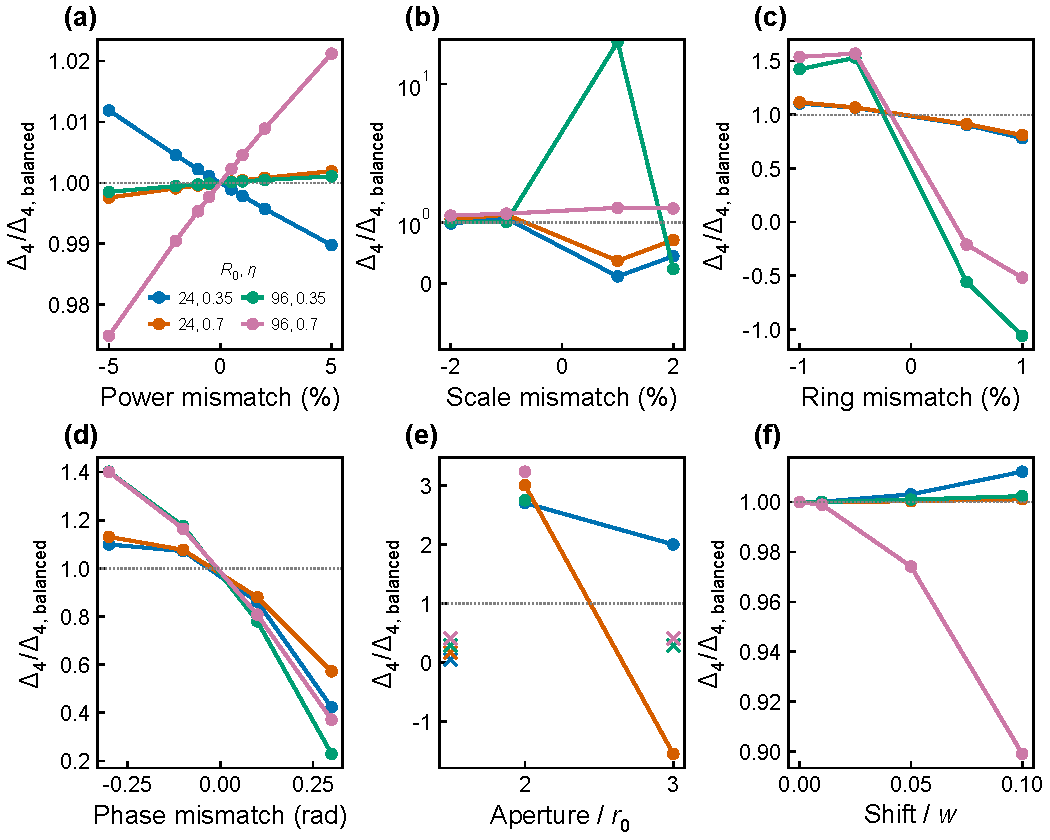
\includegraphics[width=\linewidth]{../figures/input_sensitivity.pdf}
\caption{Input sensitivity of the nominal-proxy $m=4$ advance, divided
by the corresponding balanced-input value. The legend gives $R_0,\eta$.
(a) Signed power imbalance. (b) Differential radial scale; a symmetric
logarithmic vertical axis retains large branch-dependent changes.
(c) Differential ring radius. (d) Differential quadratic phase at $r_0$.
(e) Finite source aperture; crosses denote undefined paired advances
and their vertical positions carry no numerical meaning.
(f) Displacement of the plus channel in a two-dimensional calculation.
These perturbation levels are tests, not accepted hardware tolerances.}
\label{fig:si-input}
\end{figure}

The 324 beam cases yield 315 defined selected peaks and nine cases
without a peak in the search interval, all involving the smallest source
aperture. Six further selected peaks lack a preceding half-height crossing.
In total, 309 individual half-heights and 304 paired advances are defined;
five additional differences lack the reference crossing. Missing
quantities retain separate peak, crossing, and paired-event statuses. The large change at $R_0=96$, $\eta=0.35$, positive radial
scale mismatch is retained together with its complete extrema list;
it cannot be interpreted as a small linear tolerance coefficient.

Finite source apertures can produce very weak early lobes, which remain
eligible under the declared first-peak rule. For $R_0=24$, $\eta=0.7$ and
a source aperture $3r_0$, the selected $m=1,4$ peaks occur near
$\tau=-6.11457,-5.68705$, well before the largest caustic peak. A three-level
source, radial, and axial refinement changes their last half-heights by
less than $1.3\times10^{-8}$ and their difference by less than
$2.3\times10^{-8}$. The $m=2$ preceding half-height remains missing in
that search window. Thus the large aperture-induced changes are not
interpreted as small shifts of a uniquely tracked caustic peak.

Translations are implemented by the translation invariance of the exact
scalar propagator applied to cached complex channels. The offsets are
$d/w=0,0.01,0.05,0.1$, for a shifted plus channel, opposite shifts
$\pm d/2$, or a common shift $d/2$. Nominal circular-aperture integration
uses polar quadrature with a 64,128,256-level check. Opposite half shifts
and a common half shift have equal circular-aperture channel integrals
by rotational symmetry, although their two-dimensional polarization
textures differ. This distinction prevents identical integrated values
from being mistaken for identical fields.

Elliptical inputs at $R_0=24$, $\eta=0.7$, $m=1,4$ use the area-preserving
map $(x,y)\mapsto(x/a,ay)$, $a=\exp(e/2)$, with
$e=0.005,0.01$. Both the envelope and vortex azimuth are transformed.
A signed angular Fourier expansion is propagated with the Fresnel kernel;
mode offsets $\pm16,\pm24,\pm32$ are checked. At $e=0.01$, the
omitted incident modal power outside the widest range is below
$8.3\times10^{-14}$, and the event values agree across the last two
mode ranges at saved precision. Direct two-dimensional Fresnel quadrature
at three field points, independently refining source step and angular
samples from 256 to 512, agrees with the stored modal field to relative
channel error below $9.2\times10^{-10}$, including radial interpolation.

For common ellipticity $e=0.005$, the $m=4$ advance is $0.3120567$;
at $e=0.01$ it is $0.5545883$, versus approximately $0.291969$ for
the circular input. Deforming only the plus channel at $e=0.01$ gives
$0.4195528$. Rotating the second ellipse by $90^\circ$ leaves its
circular-aperture intensity integral unchanged but changes its field map.
These results illustrate why a calibrated input shape is needed even
when total channel powers are balanced.


\section{Synthetic measurement from circular-channel counts}
\label{sec:count-measurement}
The original detector study uses the computed complex fields at $R_0=24,96$,
$\eta=0.35,0.7$, and $m=1,2,4$; the focused diagnosis below adds $m=3$
without replacing the original records. The true circular-channel intensities,
$I_\pm=|U_{m\mp1}|^2/2$, are normalized by the incident transverse power.
These are synthetic conditions; no camera, translation stage, or experimental
performance is inferred from them. Unit detection efficiency is assumed in
the reference count $N$ per axial plane. A different known efficiency can be
absorbed into $N$.

Before counting, each intensity is convolved with a circular Gaussian
point-spread function. For a radial intensity the convolution is evaluated as
\begin{equation}
 I_\sigma(r)=\int_0^\infty I(s)\frac{s}{\sigma^2}
 e^{-(r-s)^2/(2\sigma^2)} I_{0e}(rs/\sigma^2)\,\mathrm{d}s,
\end{equation}
where $I_{0e}(t)=e^{-t}I_0(t)$ is the scaled modified Bessel function.
Each square detector pixel is then integrated using $3\times3$
Gauss--Legendre quadrature. The circular aperture contains pixels whose
centres lie within the nominal proxy radius. It therefore includes finite
pixel sampling of the aperture as well as averaging within each pixel.
Tests with $5\times5$ and $7\times7$ quadrature changed the pilot half-height
positions by less than $2\times10^{-8}$ in $\tau$. The radial convolution
agreed with an independently known Gaussian-convolution solution to
$2.93\times10^{-9}$ in relative $L^2$ error.

Let $p_{\pm j}$ be the resulting fraction of incident power in pixel $j$.
The count means, before background subtraction, are
\begin{align}
 \lambda_{+j}&=N(1+g)[(1-a)p_{+j}+b p_{-j}]+B,\\
 \lambda_{-j}&=N(1-g)[a p_{+j}+(1-b)p_{-j}]+B,
 \qquad a=c+\delta/2,\quad b=c-\delta/2.
\end{align}
Independent Poisson counts and additive Gaussian read noise are generated
for the two channels. The baseline has $N=10^6$ reference counts per plane,
axial step $0.1$ mm, pixel pitch $1\,\mu$m, blur standard deviation
$1\,\mu$m, read-noise standard deviation one electron per pixel, and
background $B=0.1$ electron per pixel. The gain standard deviation is
$0.1\%$ with cross-order correlation $0.8$. The two background calibration
offsets have standard deviation $0.001$ electron per pixel and correlation
$0.5$, and are shared across scans. The mean polarimetric mixing is
$c=0.002$, with shared asymmetry standard deviation $0.0002$.
The monitor has mean $100N$ and independent Poisson noise at each plane,
shared across the compared orders.

The common axial offset has standard deviation $0.02$ mm. Independent
order-specific offsets have standard deviation $0.01$ mm, and independent
linear scan drifts have standard deviation $0.01$ mm at the scan endpoints.
For every realization, the intensity is evaluated at the displaced physical
plane while the aperture remains at its nominal position. Shifting only
the already integrated moving-aperture curve would describe a different
measurement and is not used.

Since the aperture weights are binary, the sum of independent Poisson pixel
counts is exactly Poisson with mean $\sum_j\lambda_{\pm j}$. We use this
identity to simulate the aggregate channel counts, with read variance equal
to the number of retained pixels times the per-pixel variance. This retains
the count statistics of the full image without drawing every pixel in every
realization. Representative full raw channel images and aggregate count
traces are retained in the data archive. Noise is never added as a prescribed
percentage of the final $Q$.

The scan covers $-1.5\leq\tau\leq2.5$. A cubic Savitzky--Golay filter uses
a nominal width $0.25$ in $\tau$, rounded to an odd number of samples with
at least five points. The estimator selects the largest interior smoothed
maximum within $0.2\leq\tau\leq1.8$, records all additional maxima, and
uses a three-point quadratic peak value. The half-height event is the
nearest preceding rising linear crossing. Negative counts are retained.
A missing maximum or crossing is an extraction failure; returning a number
does not imply that the correct physical peak was selected.

The linearized confidence interval propagates the full covariance through
the smoothing matrix and the peak/crossing functional. It retains
peak--crossing covariance, shared monitor and calibration errors, and
cross-order axial errors. For this simulation benchmark the covariance is
evaluated at the known expected detector signal. It is therefore an
\emph{expected-signal linearization}, not a claim that these parameters can be
estimated without calibration in an experiment. Bias and coverage are
reported separately against the ideal continuous-aperture event and the
noise-free pixel-and-blur event. Unknown systematic gain bias is not absorbed
into a random-error interval.

The design contains 96 scenarios with 1000 realizations each: marginal
sweeps of $N=10^4$--$10^7$, axial steps $0.05$--$1$ mm, gain standard
deviation $0$--$1\%$, blur $0$--$5\,\mu$m, pixel pitch
$0.5$--$4\,\mu$m, read noise $0$--$3$ electrons, and independent axial
offset $0$--$0.1$ mm, together with two predefined interacting/systematic
stress scenarios. These ranges define marginal sweeps rather than a full
Cartesian product. The scenario table reports event statuses as source data.
Four representative conditions were repeated independently with 4000
realizations. For $R_0=96$, $\eta=0.7$, $m=4$, the correct-sign fractions
were $0.251$ and $0.255$ at $N=10^6$, and $0.979$ and $0.98075$ at
$N=10^7$. These repetitions support the distinction between those two
count regimes; they do not establish a universal detection threshold.

\begin{table}[htbp]
\centering\small
\caption{Baseline synthetic measurement for $m=4$ relative to $m=1$.
Bias and interval coverage refer to the ideal continuous-aperture advance.
Widths are the full linearized 95\% interval; the correct-sign fraction is empirical.}
\label{tab:measurement-baseline}
\begin{tabular}{rrrrrrr}\toprule
$R_0$ & $\eta$ & $\Delta z_4$ (mm) & Bias (mm) & Width (mm) & Coverage & Correct sign\\\midrule
24 & 0.35 & 3.69334 & $-0.00314$ & 0.2363 & 0.957 & 1.000 \\
24 & 0.7 & 3.78726 & $-0.02302$ & 0.5604 & 0.950 & 1.000 \\
96 & 0.35 & 0.45746 & $-0.01091$ & 0.6265 & 0.955 & 0.994 \\
96 & 0.7 & 0.48972 & $-1.71029$ & 8.3827 & 0.915 & 0.251 \\
\bottomrule\end{tabular}
\end{table}

\begin{figure}[p]
\centering
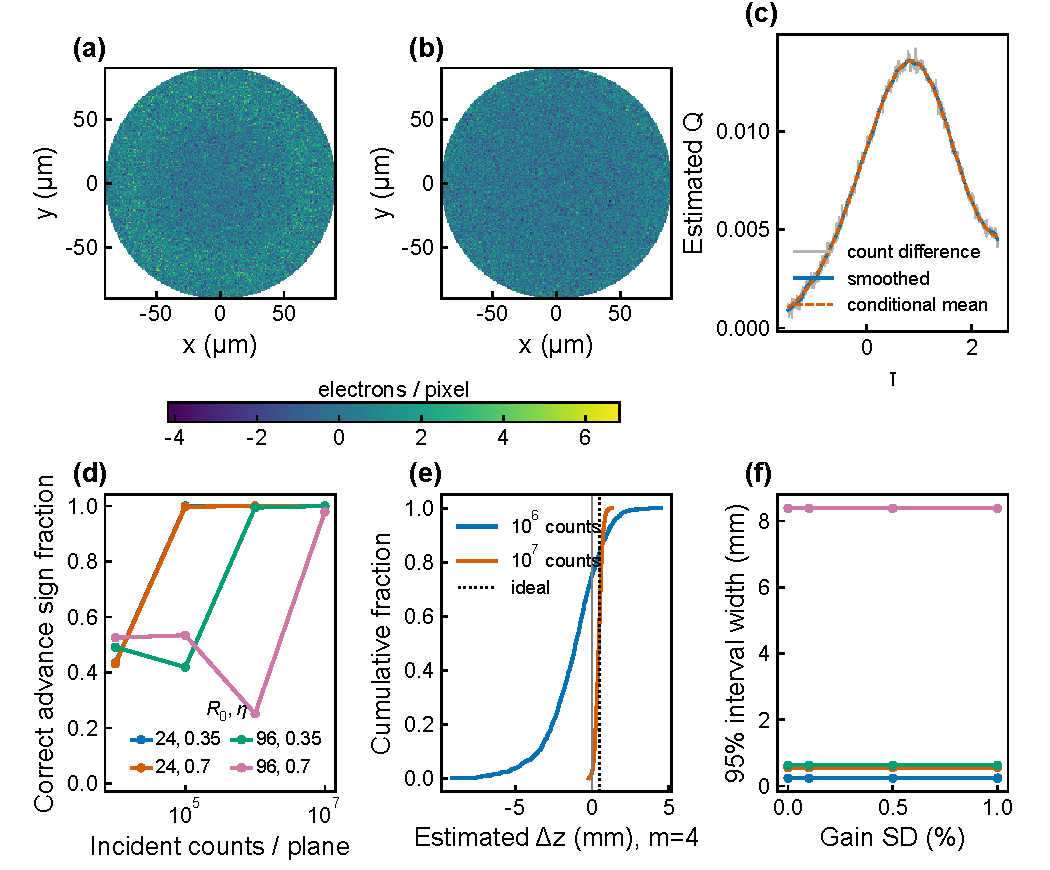
\includegraphics[width=\linewidth]{../figures/synthetic_measurement.pdf}
\caption{Synthetic count-level measurement. (a,b) Independently generated
raw circular-channel images at $\tau=0$, $R_0=24$, $\eta=0.7$, $m=4$,
with the same electron-count scale. (c) One aggregate count trace,
its smoothed estimate, and the conditional mean. (d) Correct-sign fraction
for $\Delta z_4$ in the count sweep with other conditions fixed.
(e) Full empirical cumulative distributions at $R_0=96$, $\eta=0.7$;
the dotted line is the ideal continuous-aperture advance.
(f) Linearized interval widths with the stated gain covariance.
All quantities are simulated, and each sweep point contains 1000 realizations.}
\label{fig:synthetic-measurement}
\end{figure}

For the baseline at $R_0=24$, both tested non-reference orders have the
correct advance sign in all 1000 realizations. At $R_0=96$, $\eta=0.7$,
however, the ideal $m=4$ advance is $0.48972$ mm and the estimated mean
is biased by $-1.71029$ mm. Only $25.1\%$ of realizations have the correct
sign. The failure is associated with low local counts and peak selection
under noise, rather than the absence of a mathematical crossing in the
ideal signal. In the combined low-count/coarse-image stress case,
$2.5\%$ of paired estimates cannot be extracted, while the sign fraction
among extracted estimates is approximately $0.502$. Very wide linearized
intervals in this regime are not evidence of a useful measurement.

\subsection{Four-stage failure diagnosis and frozen estimator comparison}
Before drawing the focused random samples, we fixed three extraction rules:
(i) the retained width-$0.25\tau$ blind largest-peak estimator; (ii) a
known-peak-location-assisted diagnostic using the same smoothing but selecting
the local maximum nearest the known noiseless detector peak; and (iii) one implementable blind
alternative using a pre-fixed width $0.75\tau$ and the largest peak. The
third rule uses neither the true displacement nor $D_m$. One thousand
calibration replicates determine the covariance, and 3000 independent
validation replicates determine bias, extraction, interval coverage, and
sign recovery. The protocol and seeds are stored before the validation draws.

Four stages isolate the failure. A is the continuous-field event in the
specified ROI. B applies pixel integration and blur without random noise.
C applies the fixed smoothing and peak/crossing routine to the noiseless
detector curve. D applies the same routine to the raw random channel counts.
For the difficult $R_0=96$, $\eta=0.7$, $m=4$ case, A--D give
$0.489722$, $0.484247$, $0.484237$, and $-1.242756$ mm for the retained
blind method at $N=10^6$. The imaging bias is $-0.005475$ mm and the
deterministic estimator bias is $-0.000010$ mm, whereas the random bias from
C to D is $-1.726993$ mm. The original 1000- and 4000-realization results
are therefore corroborated without being overwritten.

The estimator returns a number in every focused validation scan, so all-run
and extracted-only fractions coincide here. At $N=10^6$, the retained blind
and location-assisted rules select the same discrete local maximum in only
$14.9\%$, $13.6\%$, and $13.0\%$ of the $m=2,3,4$ scans. Equality of these
sample indices does not establish that either selected the same physical peak
branch. The retained rule gives correct-sign fractions of $42.0\%$, $32.0\%$,
and $25.7\%$; the location-assisted diagnostic gives only $47.4\%$, $42.7\%$,
and $38.4\%$. This diagnostic uses the noiseless peak location but leaves the
noisy peak value, physical branch, and rising crossing free, so its residual
error cannot be attributed uniquely to the crossing. The wider blind rule
improves the fractions to $50.9\%$, $52.5\%$, and $54.9\%$, still insufficient
for a feasibility claim.

At the detector half-height and $N=10^6$, the expected $(I_+,I_-)$ ROI
counts are $(85.81,6.83)$ for $m=1$ and $(163.44,29.75)$ for $m=4$.
The aperture contains hundreds to thousands of pixels depending on order,
so one electron of independent read noise per pixel accumulates in the
aggregate. A Poisson-only ablation gives retained-estimator sign fractions
$68.9\%$, $85.1\%$, and $94.0\%$ for $m=2,3,4$. Counting plus read noise
reduces them to $43.5\%$, $37.1\%$, and $26.9\%$, reproducing most of the
full failure; counting plus background alone gives $57.5\%$, $65.2\%$,
and $67.3\%$. Hence the dominant modeled cause is accumulated read noise,
with peak/crossing selection converting it into order-dependent bias;
background adds degradation. It is not accurately described as incident
photon shortage alone.

At $N=10^7$, the retained estimator gives correct signs in $74.6\%$,
$91.9\%$, and $97.6\%$ of the $m=2,3,4$ scans, and the pre-fixed wider
rule gives $86.5\%$, $99.1\%$, and $99.9\%$. The smaller $m=2$ shift
remains more difficult. At $R_0=24$ and $N=10^6$, all $m=2,3,4$ signs
are recovered for both tested apodizations under the retained estimator.
These outcomes are conditional on the stated synthetic detector and do not
set a general photon or hardware threshold.

\begin{table}[htbp]
\centering\scriptsize
\caption{Four-stage diagnosis at $R_0=96$, $\eta=0.7$, and $N=10^6$ for the retained blind estimator. A is the continuous-field event, B includes noiseless pixel and blur response, C applies the fixed smoothing and peak rule to B, and D is the mean over 3000 independent count-level validation scans. Values are millimeters except the final percentage.}
\label{tab:measurement-stages}
\begin{tabular}{r@{\quad}rrrrrrrr}
\toprule
$m$ & A & B & C & D & B$-$A & C$-$B & D$-$C & sign (\%) \\
\midrule
2 & 0.149997 & 0.137186 & 0.137255 & $-0.304859$ & $-0.012811$ & $+0.000069$ & $-0.442114$ & 42.0 \\
3 & 0.314388 & 0.311861 & 0.311892 & $-0.715232$ & $-0.002527$ & $+0.000030$ & $-1.027124$ & 32.0 \\
4 & 0.489722 & 0.484247 & 0.484237 & $-1.242756$ & $-0.005475$ & $-0.000010$ & $-1.726993$ & 25.7 \\
\bottomrule
\end{tabular}
\end{table}

\begin{table}[htbp]
\centering\scriptsize
\caption{Estimator comparison for the difficult $R_0=96$, $\eta=0.7$ condition. Sign percentages and random-mean advances use 3000 independent validation scans. The location-assisted diagnostic selects the noisy local maximum nearest the known noiseless peak location; it does not fix the noisy peak value, physical branch, or half-height crossing. The wide estimator is a pre-frozen blind rule.}
\label{tab:measurement-estimators}
\begin{tabular}{rcrrr@{\qquad}rrr}
\toprule
& & \multicolumn{3}{c}{correct sign (\%)} & \multicolumn{3}{c}{mean advance (mm)}\\
$N$ & estimator & $m=2$ & $m=3$ & $m=4$ & $m=2$ & $m=3$ & $m=4$ \\
\midrule
$10^{6}$ & current & 42.0 & 32.0 & 25.7 & $-0.305$ & $-0.715$ & $-1.243$ \\
$10^{6}$ & location assisted & 47.4 & 42.7 & 38.4 & $-0.119$ & $-0.315$ & $-0.590$ \\
$10^{6}$ & wide & 50.9 & 52.5 & 54.9 & 0.048 & 0.071 & 0.135 \\
$10^{7}$ & current & 74.6 & 91.9 & 97.6 & 0.126 & 0.289 & 0.449 \\
$10^{7}$ & location assisted & 73.3 & 91.4 & 97.7 & 0.130 & 0.302 & 0.473 \\
$10^{7}$ & wide & 86.5 & 99.1 & 99.9 & 0.132 & 0.303 & 0.473 \\
\bottomrule
\end{tabular}
\end{table}


\begin{figure}[p]
\centering
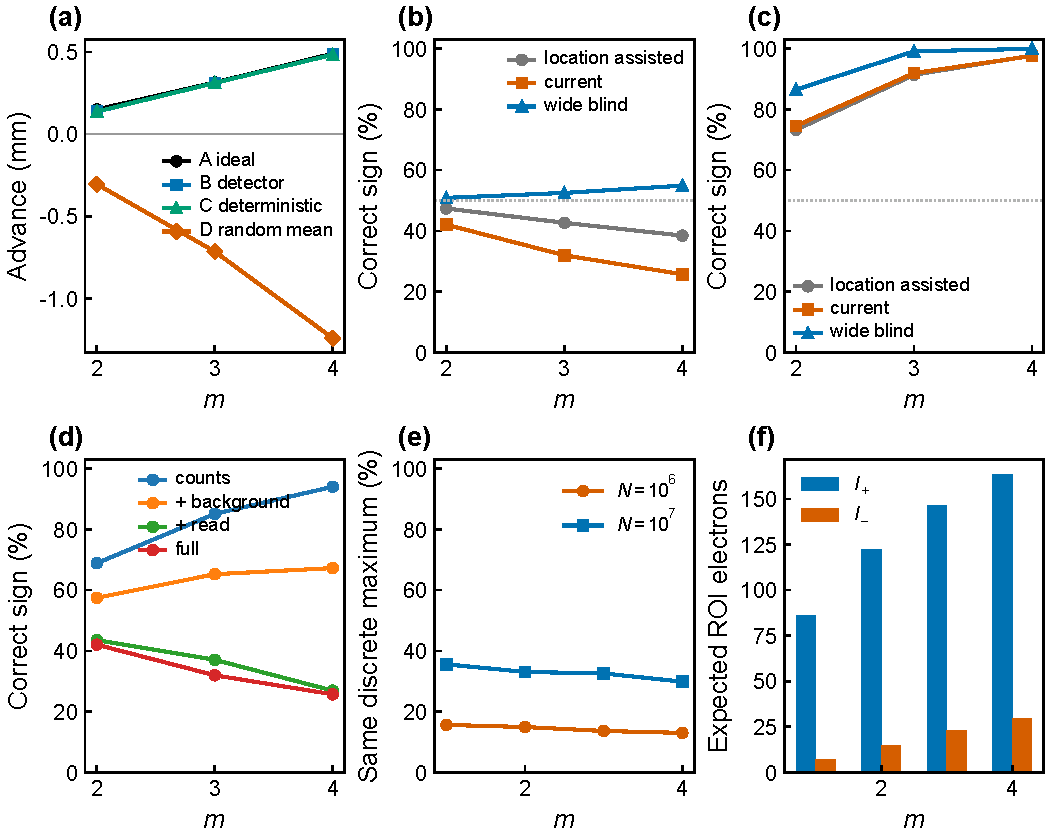
\includegraphics[width=\linewidth]{../figures/focused_measurement_diagnosis.pdf}
\caption{Focused diagnosis of the difficult $R_0=96$, $\eta=0.7$
measurement. (a) Continuous-field (A), noiseless detector (B), deterministic
estimator (C), and random validation mean (D) for the retained blind rule.
(b,c) Correct-sign fractions for the location-assisted diagnostic, retained blind, and pre-fixed wider
blind estimators at $10^6$ and $10^7$ reference counts per plane.
(d) Noise-source ablations at $10^6$ counts for the retained estimator.
(e) Fraction for which the retained blind and location-assisted rules select
the same discrete local maximum; this is not a physical peak-identity label.
(f) Expected circular-channel ROI counts at
the noiseless detector half-height for $10^6$ incident reference counts.
Each focused fraction uses 3000 independent validation scans; the assisted
rule is diagnostic and the wider blind rule was fixed before those scans.}
\label{fig:focused-measurement}
\end{figure}
\FloatBarrier

\subsection{Proposed channel-resolved optical implementation}

Figure~\ref{fig:proposed-experiment} maps the modeled observable to a
laboratory measurement. A linearly polarized continuous-wave source at
$632.8$~nm is spatially filtered and expanded before a polarization
Mach--Zehnder interferometer. The two arms use phase-only spatial-light-
modulator holograms with Fourier filtering to encode the same finite-energy
circular Airy envelope $f_{\mathrm A}(r)$ and the charges $q_+=m-1$ and
$q_-=m+1$. A half-wave plate and the hologram efficiencies set the incident
channel powers. The arms are recombined in orthogonal linear polarizations;
a quarter-wave plate at $45^\circ$ converts them to the circular basis used in
the main text. A uniform inter-arm phase changes the polarization
orientation but not $I_\pm$ or $S_3$. Transverse registration, equal radial
scale, and power balance must nevertheless be calibrated because they change
the measured channel intensities.

The acquisition head is translated through the autofocusing region, or an
equivalent translated relay images each plane. A quarter-wave plate followed
by a polarizing beam splitter sends the two circular components to synchronized
detectors. A monitor photodiode records the incident normalization. Full frames
are retained, so the scaled proxy boundary is applied digitally with physical
radius
\begin{equation}
 \rho_s(z)=\frac{2kw^3x_s}{z},\qquad x_s=j'_{m,1},
\end{equation}
rather than with a moving mechanical iris. After dark, flat-field, gain,
polarimetric-leakage, and image-registration corrections, let
$\widetilde C_{\pm j}(z)$ denote the corrected count in pixel $j$. The directly
measured traces are
\begin{align}
 \widehat Q(z)&=\frac{1}{\widehat P_{\rm in}(z)}
  \sum_{j\in{\rm ROI}(z)}[\widetilde C_{+j}(z)-\widetilde C_{-j}(z)],\\
 \widehat T(z)&=\frac{1}{\widehat P_{\rm in}(z)}
  \sum_{j\in{\rm ROI}(z)}[\widetilde C_{+j}(z)+\widetilde C_{-j}(z)],
 \qquad
 \widehat{\bar p}_3(z)=\frac{\widehat Q(z)}{\widehat T(z)}.
\end{align}
The same fixed peak and rising-crossing rules used in the count simulation
then give $z_{50}(m)$ and $\Delta z_m=z_{50}(1)-z_{50}(m)$. For the alternative
actual-zero analysis, the first positive-to-negative zero is extracted from
the calibrated, azimuthally averaged $S_3$ map at each plane and its branch
status is retained. The axial scan increment is only the sampling interval;
repeat scans and the calibrated covariance are required to determine event
uncertainty.

Input certification is kept separate from this primary acquisition. A
quarter-wave plate and rotating linear polarizer provide full-Stokes images,
whereas interference of each circularly selected component with a matched
spherical reference checks $q_+$ and $q_-$. A linear-analyzer petal pattern is
not used to infer $m$, because the fixed $P=1$ family has the same twofold
modulation for every $m$. These modules follow established SLM preparation,
Stokes-polarimetry, and circular-channel interferometry procedures
\cite{Liu2021,Yan2025,Zhu2025}. Figure~\ref{fig:proposed-experiment} is an
implementable proposal; the present work has not built this apparatus, and the
feasibility numbers above remain predictions of the stated detector model.

\begin{figure}[p]
\centering
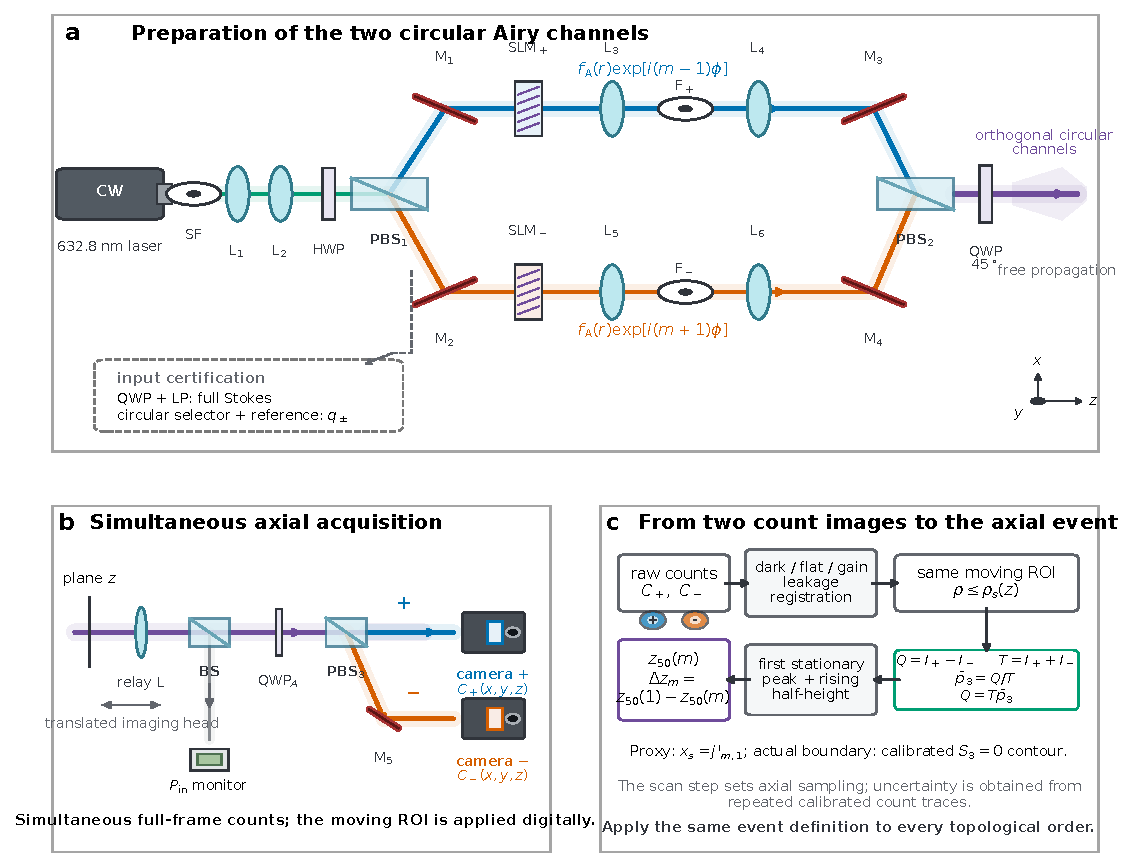
\includegraphics[width=\linewidth]{../figures/proposed_experimental_layout.pdf}
\caption{Proposed measurement of the topological-order-dependent axial event.
(a) A polarization Mach--Zehnder interferometer prepares the same circular
Airy envelope in the $q_+=m-1$ and $q_-=m+1$ arms and converts the recombined
field to orthogonal circular polarizations. The dashed branch contains
independent input diagnostics. SF, spatial filter; L1--L2, beam expander; HWP,
half-wave plate; PBS, polarizing beam splitter; SLM, spatial light modulator;
QWP, quarter-wave plate. (b) A translated imaging head separates and records
the two circular-channel count images simultaneously while a photodiode
monitors incident power. (c) Calibrated full-frame counts are integrated in
the digital moving ROI to obtain $Q$, $T$, and $\bar p_3$ before the fixed
peak and rising-half-height estimator is applied. This is a proposed optical
implementation, not an experiment performed in the present work.}
\label{fig:proposed-experiment}
\end{figure}


\FloatBarrier
\section{Finite radius residual
mechanism}\label{finite-radius-residual-mechanism}

\subsubsection*{The Airy convolution}\label{the-airy-convolution}

For \(\alpha>0\) define the one-dimensional Fresnel propagation of the
apodized Airy function:

\begin{equation}F(y,\zeta)=\frac{1}{\sqrt{2\pi i\zeta}}\int_{-\infty}^{\infty}\operatorname{Ai}(t)e^{\alpha t}e^{i(y-t)^2/(2\zeta)}\,\mathrm{d}t.\end{equation}

The initial profile has Fourier transform \(\exp[(\alpha-ik)^3/3]\).
Multiplication by \(\exp(-i\zeta k^2/2)\) and completion of the cubic
phase give

\begin{equation}F(y,\zeta)=\operatorname{Ai}(y-\zeta^2/4+i\alpha\zeta)e^{\Phi(y,\zeta)},\end{equation}

\begin{equation}\Phi(y,\zeta)=\alpha(y-\zeta^2/2)+i[\zeta(y+\alpha^2)/2-\zeta^3/12].\end{equation}

This is the finite-energy Airy solution of Siviloglou and
Christodoulides, Eq. (5) {[}4{]}. Setting \(t=R_0-s\), \(a=R\cos\theta\)
and \(y=R_0-a\) converts the full-line source integral without its
factor \(s\) to
\(\sqrt{2\pi i\zeta}\,e^{-ia^2/(2\zeta)}F(R_0-a,\zeta)\). Applying
\(i\zeta\partial_a\) restores the factor \(s\). The sign follows
directly by differentiating \(\exp(-ias/\zeta)\).

For integer \(q\), the Bessel angular identity {[}5{]} is

\begin{equation}J_q(v)=\frac{i^q}{2\pi}\int_0^{2\pi}e^{-iv\cos\theta}e^{iq\theta}\,\mathrm{d}\theta.\end{equation}

Let \(X=R_0-\zeta^2/4+i\alpha\zeta\). After removing a nonzero common
factor and normalizing by \(\zeta^2/2\), the angular field is

\begin{equation}\mathcal H_q=\frac{1}{2\pi}\int_0^{2\pi}e^{iq\theta}G(a,\zeta)\left[B(a,\zeta)\operatorname{Ai}(X-a)-\frac{2i}{\zeta}\operatorname{Ai}'(X-a)\right]\,\mathrm{d}\theta,\end{equation}

\begin{equation}G(a,\zeta)=e^{-i\zeta a/2-\alpha a-ia^2/(2\zeta)},\qquad B(a,\zeta)=1-\frac{2i\alpha}{\zeta}+\frac{2a}{\zeta^2}.\end{equation}

The normalized proxy signal is therefore

\begin{equation}\widetilde Q_m=\frac{V e^{-2\eta\tau\epsilon-\eta\tau^2\epsilon^3/2}}{I_{0,m}}\int_0^{b_m}x\left(|\mathcal H_{m-1}|^2-|\mathcal H_{m+1}|^2\right)\,\mathrm{d}x,\end{equation}

where \(\epsilon=R_0^{-1/2}\), \(V=1+\tau\epsilon^2/2\) and
\(I_{0,m}=2mJ_m^2(b_m)\). This normalization differs from \(Q_m\) by a
positive factor independent of \(\tau\), so it leaves peaks and
half-height events unchanged. The \(V\) and exponential factors must
remain during event extraction.

For reduced R-S propagation, use \(d\) instead of \(\zeta\) inside
\(\mathcal H_q\). Since \(d\) depends on \(x\), its signal prefactor
must be kept inside the \(x\) integral:

\begin{equation}W_{\mathrm{RS}}(x)=\frac{d\epsilon}{2}e^{-2\eta\tau\epsilon-\eta\tau^2\epsilon^3/2-\alpha(R/kw)^2},\end{equation}

\begin{equation}\widetilde Q_m^{\mathrm{RS}}=\frac{1}{I_{0,m}}\int_0^{b_m}xW_{\mathrm{RS}}(x)\left(|\mathcal H_{m-1}(d)|^2-|\mathcal H_{m+1}(d)|^2\right)\,\mathrm{d}x.\end{equation}

This expression retains the exact geometry of the manuscript's reduced
kernel. It is not a full Maxwell or unexpanded Rayleigh-Sommerfeld
calculation. The angular identity sums the complete field coherently and
introduces no arbitrary spectral partition.

\subsubsection*{Controlled negative-source
extension}\label{controlled-negative-source-extension}

Replacing the physical interval \(s\geq0\) by the full real line adds an
integral over \(s=-v<0\). Since \(|J_q(t)|\leq1\) for real \(t\) and
integer \(q\), the positive-axis Airy bound {[}6{]} and convexity of
\((R_0+v)^{3/2}\) give, for \(\alpha<\sqrt{R_0}\),

\begin{equation}|\delta I_q|\leq\frac{e^{\alpha R_0-2R_0^{3/2}/3}}{2\sqrt\pi R_0^{1/4}(\sqrt{R_0}-\alpha)^2}.\end{equation}

Indeed, \(\operatorname{Ai}(u)\leq e^{-2u^{3/2}/3}/(2\sqrt\pi u^{1/4})\)
for \(u>0\), and \(2(R_0+v)^{3/2}/3\geq2R_0^{3/2}/3+\sqrt{R_0}v\). The
remaining integral is \(\int_0^\infty v e^{-(\sqrt{R_0}-\alpha)v}\,\mathrm{d}v\).
The resulting dimensionless source-integral bounds are
\(1.1541\times10^{-36}\) at \(R_0=24\), \(4.8580\times10^{-76}\) at 40
and \(2.433\times10^{-275}\) at 96. These are bounds before the known
propagation prefactor, not estimates obtained from cancellation. This
artificial extension cannot account for the observed \(10^{-2}\) changes
in \(R_0\Delta\).

\subsection{Coefficients and event
recursion}\label{coefficients-and-event-recursion}

The angular formula admits direct expansion around \(\epsilon=0\). In
the Fresnel case,

\begin{equation}a=\frac{\epsilon x\cos\theta}{V},\quad X=-\tau+i\eta+\epsilon^2(-\tau^2/4+i\eta\tau/2),\quad \zeta a/2=x\cos\theta.\end{equation}

Expand \(V^{-1}\) geometrically, the two remaining exponentials by
power-series multiplication, and \(\operatorname{Ai}(X-a)\) about
\(-\tau+i\eta\). Its derivatives satisfy
\(A^{(k)}=XA^{(k-2)}+(k-2)A^{(k-3)}\) for \(k\geq3\), with \(A''=XA\).
The field coefficients \(H_{q,n}\) then determine every intensity
coefficient by the convolution \(\sum_{j=0}^{n}H_{q,j}H_{q,n-j}^*\). The
common signal prefactor is convolved at the same total order. There is
no truncation by derivative number followed by uncontrolled squaring.

Write \(Q_m(\tau,\epsilon)=\sum_n q_{m,n}(\tau)\epsilon^n\),
\(p_m=p_0+\sum_{n\geq1}p_{m,n}\epsilon^n\) and
\(h_m=h_0+\sum_{n\geq1}h_{m,n}\epsilon^n\). For a simple peak and rising
crossing, coefficient extraction gives

\begin{equation}p_{m,n}=-\frac{[\epsilon^n]\,\partial_\tau Q_m(p_0+\sum_{j<n}p_{m,j}\epsilon^j,\epsilon)}{q_{m,0}''(p_0)},\end{equation}

\begin{equation}h_{m,n}=\frac{\tfrac12[\epsilon^n]Q_m(p_0+\sum_{j<n}p_{m,j}\epsilon^j,\epsilon)-[\epsilon^n]Q_m(h_0+\sum_{j<n}h_{m,j}\epsilon^j,\epsilon)}{q_{m,0}'(h_0)}.\end{equation}

The unknown \(p_{m,n}\) does not enter the peak height at this order
because \(q_{m,0}'(p_0)=0\). This proves the recursion under its
nondegeneracy assumptions. The coefficients \(c_n=h_{1,n}-h_{3,n}\) are
fixed by the model and event definition. They do not depend on a chosen
set of propagation radii. The normalized full-line signal is analytic
locally in \(\epsilon\) where \(V\neq0\); the implicit function theorem
supplies local analytic events while their denominators remain nonzero.
The source extension contributes a beyond-all-orders term to the
physical half-line integral. These local facts alone do not certify a
global convergence radius for the event series.

\Needspace{18\baselineskip}
\begin{longtable}[]{@{}lrlr@{}}
\caption{Analytic event-difference coefficients for $m=3$ relative to $m=1$ at $\eta=0.35$, with $\Delta=\sum_n c_n\epsilon^n$ and $\epsilon=R_0^{-1/2}$. The first-order coefficient vanishes analytically.}\label{tab:event-series-coefficients}\\
\toprule\noalign{}
\(n\) & \(c_n\) & \(n\) & \(c_n\) \\
\midrule\noalign{}
\endhead
\bottomrule\noalign{}
\endlastfoot
2 & 4.41467828893 & 3 & $-1.44016807989$ \\
4 & 2.58765834920 & 5 & 3.36680299947 \\
6 & 13.3529860411 & 7 & 21.1128977205 \\
8 & $-49.8888463954$ & 9 & 91.5175673968 \\
10 & 237.809936151 & 11 & $-385.651361911$ \\
12 & 738.534340134 & 13 & $-809.692872335$ \\
14 & 3130.68031359 & 1 & 0 analytically \\
\end{longtable}

The computed \(c_1\) is \(1.2\times10^{-15}\). The first three nonzero
coefficients reproduce the independent earlier fold derivation. Changing
the Cauchy derivative-contour radius from 0.7 to 0.9 changes no
coefficient through order 14 by more than \(8.3\times10^{-10}\).
Separate order-10 checks refine the radial and angular quadratures from
32/64 to 48/96 nodes. Cauchy extraction evaluates derivatives of an
analytic formula; it does not fit propagated event values.

\subsection{Why the minimum was
missed}\label{why-the-minimum-was-missed}

The scaled event series is \(R_0\Delta=\sum_{n\geq2}c_n R_0^{1-n/2}\).
At fourth order it contains only \(A_3+B_3/\sqrt{R_0}+C_3/R_0\). Its
stationary point is \((2C_3/|B_3|)^2=12.91361\), outside the observed
intermediate-radius minimum. Adding the positive fifth- and sixth-order
terms shifts the minimum toward the full calculation.

\begin{longtable}[]{@{}lrr@{}}
\caption{Minimum of the scaled advance $R_0\Delta$ for successive event-series truncations and the full propagation models at $m=3$, $\eta=0.35$. Truncation order denotes the power of $\epsilon$.}\label{tab:minimum-truncation}\\
\toprule\noalign{}
Event truncation & Predicted minimum \(R_0\) & Minimum \(R_0\Delta\) \\
\midrule\noalign{}
\endhead
\bottomrule\noalign{}
\endlastfoot
4 & 12.91361 & 4.21429595 \\
5 & 24.97050 & 4.25708537 \\
6 & 34.41707 & 4.27232531 \\
8 & 35.78792 & 4.27406412 \\
10 & 36.41148 & 4.27452784 \\
12 & 36.37256 & 4.27450296 \\
14 & 36.37128 & 4.27450221 \\
Full Fresnel & 36.37127 & 4.27450221 \\
Reduced R-S & 36.37130 & 4.27450539 \\
\end{longtable}

These are order controls without coefficient fitting. The high orders do
not merely improve a regression statistic: they predict the location and
depth of the minimum and the sign of its curvature. The decomposition
below additionally identifies which operations generate the missing
terms.

For each order \(n\), split the new signal coefficient into (i)
\(H_0H_n^*+H_nH_0^*\), (ii) lower-field products and the common
prefactor, and (iii) inherited nonlinear terms from the two implicit
event equations. Applying the linear crossing functional
\([q_n(p_0)/2-q_n(h_0)]/q_0'(h_0)\) to (i) and (ii), and assigning the
remainder of \(h_n\) to (iii), gives the following exact algebraic
grouping in this declared expansion convention.

\begin{longtable}[]{@{}
  >{\raggedright\arraybackslash}p{(\linewidth - 8\tabcolsep) * \real{0.1579}}
  >{\raggedleft\arraybackslash}p{(\linewidth - 8\tabcolsep) * \real{0.2105}}
  >{\raggedleft\arraybackslash}p{(\linewidth - 8\tabcolsep) * \real{0.2105}}
  >{\raggedleft\arraybackslash}p{(\linewidth - 8\tabcolsep) * \real{0.2105}}
  >{\raggedleft\arraybackslash}p{(\linewidth - 8\tabcolsep) * \real{0.2105}}@{}}
\caption{Signed contributions to the fifth- and sixth-order event coefficients at $m=3$, $\eta=0.35$, using the field-product and implicit-event grouping defined in the text.}\label{tab:event-coefficient-decomposition}\\
\toprule\noalign{}
\begin{minipage}[b]{\linewidth}\raggedright
Order
\end{minipage} & \begin{minipage}[b]{\linewidth}\raggedleft
New field term
\end{minipage} & \begin{minipage}[b]{\linewidth}\raggedleft
Lower products and prefactor
\end{minipage} & \begin{minipage}[b]{\linewidth}\raggedleft
Nonlinear event terms
\end{minipage} & \begin{minipage}[b]{\linewidth}\raggedleft
Total \(c_n\)
\end{minipage} \\
\midrule\noalign{}
\endhead
\bottomrule\noalign{}
\endlastfoot
5 & 1.04031657 & 23.80479484 & $-21.47830841$ & 3.36680300 \\
6 & 22.98782712 & 54.38661509 & $-64.02145617$ & 13.35298604 \\
\end{longtable}

The large signed cancellations rule out interpreting \(c_5\) or \(c_6\)
as the power carried by a separate branch. They are coherent
finite-radius field corrections processed through peak normalization and
a moving half-height. As an event control, forcing the target's
normalization peak to the reference peak changes \(R_0\Delta\) to
4.52744, 4.42926 and 4.36945 at 24, 40 and 96; the dip over these three
points disappears. This artificial control isolates the importance of
the peak condition but is not proposed as a replacement observable.
Removing \(c_5\) or \(c_6\) from the fixed analytic series likewise
displaces the minimum; all values are retained in
coefficient\_decomposition.json.

\subsection{Predictions and independent numerical
evidence}\label{predictions-and-independent-numerical-evidence}

All coefficients were generated solely from the analytic identity; the
generators never load propagation data. Predictions at the new radii
were evaluated with these fixed coefficients. New controls are
\(R_0=20,28,36,44,48,64,80\); the report also recomputes the original
radii and extends to 256. The maximum fourteenth-order error in
\(R_0\Delta\) against the full Fresnel identity on the new controls is
\(2.84\times10^{-7}\), attained at 20. Over sampled \(24\leq R_0\leq96\)
it is below \(7.1\times10^{-8}\). The small reduced R-S/Fresnel
difference is retained separately, rather than absorbed into a fitted
high-order term.

\begin{longtable}[]{@{}
  >{\raggedright\arraybackslash}p{(\linewidth - 6\tabcolsep) * \real{0.2000}}
  >{\raggedleft\arraybackslash}p{(\linewidth - 6\tabcolsep) * \real{0.2667}}
  >{\raggedleft\arraybackslash}p{(\linewidth - 6\tabcolsep) * \real{0.2667}}
  >{\raggedleft\arraybackslash}p{(\linewidth - 6\tabcolsep) * \real{0.2667}}@{}}
\caption{Scaled reduced R-S advance, fourteenth-order Fresnel event-series error, and reduced R-S minus Fresnel difference at $m=3$, $\eta=0.35$. All advances are relative to $m=1$.}\label{tab:residual-model-comparison}\\
\toprule\noalign{}
\begin{minipage}[b]{\linewidth}\raggedright
\(R_0\)
\end{minipage} & \begin{minipage}[b]{\linewidth}\raggedleft
Reduced R-S \(R_0\Delta\)
\end{minipage} & \begin{minipage}[b]{\linewidth}\raggedleft
Fourteenth-order Fresnel error in \(R_0\Delta\)
\end{minipage} & \begin{minipage}[b]{\linewidth}\raggedleft
R-S minus Fresnel
\end{minipage} \\
\midrule\noalign{}
\endhead
\bottomrule\noalign{}
\endlastfoot
24 & 4.286137374 & \(+7.02\times10^{-8}\) & \(3.225\times10^{-6}\) \\
36 & 4.274510642 & \(-2.94\times10^{-9}\) & \(3.178\times10^{-6}\) \\
40 & 4.274925216 & \(-2.94\times10^{-9}\) & \(3.172\times10^{-6}\) \\
48 & 4.277668295 & \(-1.75\times10^{-9}\) & \(3.166\times10^{-6}\) \\
64 & 4.285437979 & \(-4.95\times10^{-10}\) & \(3.161\times10^{-6}\) \\
96 & 4.299868386 & \(-5.99\times10^{-11}\) & \(3.161\times10^{-6}\) \\
\end{longtable}

The angular implementation uses Gauss-Legendre integration in \(x\) and
periodic trapezoidal integration in angle. The independent
positive-source implementation evaluates the original oscillatory radial
integral by composite Gauss-Legendre quadrature, with exact reduced R-S
geometry and without a spectral transform, phase expansion, radial
interpolation or axial spline. Separate tests halve the source panels
and extend the exponential cutoff. Refining panels from 0.5 to 0.25 and
cutoff from 22 to 26 changes the scaled advance by at most
\(4.64\times10^{-10}\). The finest direct-source results differ from the
compact reduced R-S evaluation by at most \(1.41\times10^{-12}\) in
\(R_0\Delta\). The arbitrary precision implementation uses a third
angular evaluation: an Airy Taylor series in \(a\) and analytic angular
moments expressed as Bessel derivatives. It uses mpmath at 35 and 50
decimal digits, 20/28 radial nodes and 36/48 angular-series terms. At
the two event locations for each of \(m=1,3\) and \(R_0=24,40,96\), the
maximum signal difference between these precision settings is
\(6.0\times10^{-33}\); the double-precision angular implementation
differs by at most \(1.45\times10^{-15}\). These are measured numerical
differences, not interval-certified bounds.

The first peaks and preceding rising crossings continue smoothly across
the 16 tested radii from 16 to 256. The minimum crossing slope of the
normalized signal is 0.1035; the minimum magnitude of the selected peak
curvature is 0.2561. All detected later maxima are retained in
event\_continuation.csv. The selected first maxima remain separated from
them. Thus the tested minimum is not associated with a detected event
switch, peak degeneracy or a selected-zero jump.

\begin{figure}
\centering
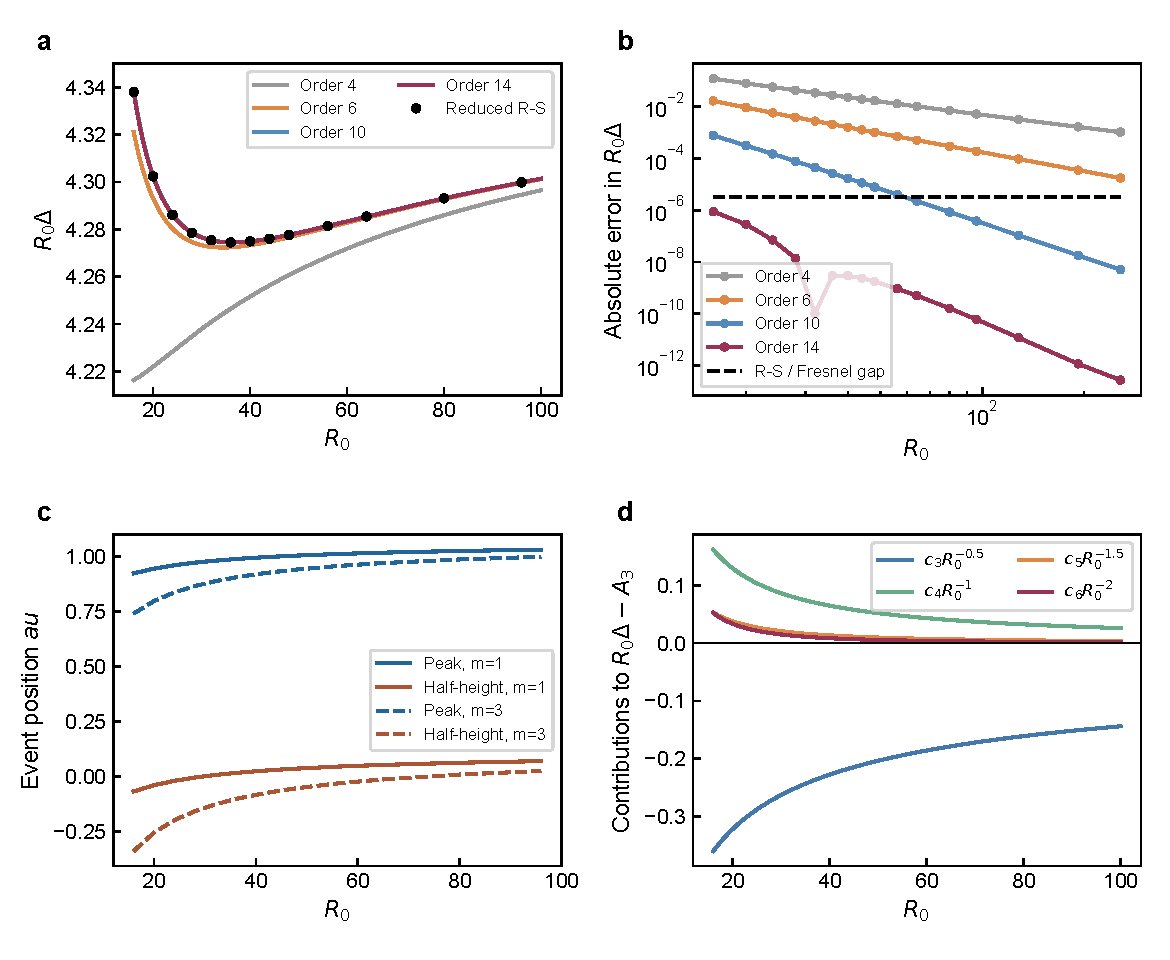
\includegraphics[width=5.25in,height=\textheight,keepaspectratio]{../figures/residual_mechanism.pdf}
\caption{Mechanism evidence. (a) Non-fitted event expansions
and full reduced R-S values. (b) Truncation errors against the full
Fresnel identity and the separately retained geometry correction. (c)
First peak and rising half-height continuation. (d) Signed lower-order
contributions to the scaled advance.}
\end{figure}

\subsection{Error accounting and
interpretation}\label{error-accounting-and-interpretation}

The signed residual admits the exact bookkeeping identity

\begin{equation}\Delta_{\mathrm{RS}}-\Delta_4=(\Delta_{\mathrm{RS}}-\Delta_{\mathrm F})+\sum_{n=5}^{14}c_nR_0^{-n/2}+(\Delta_{\mathrm F}-\Delta_{14}).\end{equation}

The first term is the model geometry correction, the second is the
analytic high-order event contribution and the third is the retained
series remainder. The source-extension bound and numerical evaluation
error are reported separately. This identity closes the residual without
allocating coherent powers to arbitrary spectral windows.

\begin{longtable}[]{@{}
  >{\raggedright\arraybackslash}p{(\linewidth - 4\tabcolsep) * \real{0.3333}}
  >{\raggedright\arraybackslash}p{(\linewidth - 4\tabcolsep) * \real{0.3333}}
  >{\raggedright\arraybackslash}p{(\linewidth - 4\tabcolsep) * \real{0.3333}}@{}}
\caption{Source-extension, numerical, finite-series, and model-geometry contributions to the residual analysis for $m=3$, $\eta=0.35$. Numerical differences and the analytic bound are reported separately.}\label{tab:residual-error-accounting}\\
\toprule\noalign{}
\begin{minipage}[b]{\linewidth}\raggedright
Contribution
\end{minipage} & \begin{minipage}[b]{\linewidth}\raggedright
Evidence and scale
\end{minipage} & \begin{minipage}[b]{\linewidth}\raggedright
Interpretation
\end{minipage} \\
\midrule\noalign{}
\endhead
\bottomrule\noalign{}
\endlastfoot
Source extension & Analytic bound \(1.16\times10^{-36}\) on \(I_q\) at
24 & Rigorous positive-source extension control \\
Angular and radial quadratures & 48/96 to 72/128 nodes: scaled-advance
change below \(6.2\times10^{-14}\) & Measured numerical convergence \\
Independent source quadrature & Source refinement change below
\(4.64\times10^{-10}\) in scaled advance & Direct check of the original
integral \\
Arbitrary precision signal evaluation & Maximum double/50-digit
difference \(1.45\times10^{-15}\) & Independent Airy/Bessel
implementation \\
Fourteenth-order remainder & Below \(7.1\times10^{-8}\) in sampled
\(R_0\Delta\), 24--96 & Finite-order approximation, not quadrature
noise \\
Reduced R-S versus Fresnel & \(3.16\)--\(3.23\times10^{-6}\) in
\(R_0\Delta\), 24--96 & Separate kernel geometry correction \\
Observed dip and recovery & 24 to 40: \(-0.01121216\); 40 to 96:
\(+0.02494317\) & Resolved finite-radius behavior \\
\end{longtable}

For the reduced R-S model and fixed-proxy half-height event, the independently derived higher-order terms quantitatively account for the minimum. The peak and crossing branches remain continuous over the sampled radii. A decomposition into inward, outward, and endpoint powers remains representation dependent.


\bibliographystyle{unsrtnat}
\bibliography{../manuscript/references}
\begin{enumerate}\setcounter{enumi}{3}
\item G. A. Siviloglou and D. N. Christodoulides, Opt. Lett. 32, 979--981 (2007), \linebreak doi: 10.1364/OL.32.000979.
\item NIST DLMF, Sections 9.5 and 10.9.2, \url{https://dlmf.nist.gov/10.9.E2}.
\item NIST DLMF, Equation 9.7.15, \url{https://dlmf.nist.gov/9.7.E15}.
\end{enumerate}
\end{document}
